\documentclass[12pt,a4paper]{article}

\usepackage{amsmath}
\usepackage[utf8]{inputenc}
\usepackage{amsmath}
\usepackage{amsfonts}
\usepackage{amssymb}
\usepackage{calrsfs}
\usepackage[left=2cm,right=2cm,top=2cm,bottom=2cm]{geometry}
\usepackage[mathscr]{euscript}

\usepackage{graphicx}
\usepackage{subcaption}

%%%for typing bold nubers%%%%%%%%
\usepackage{bm}
%%%%%%%%%%%%%%%%%%%%%%%%%%%%%%%%%

%%%%%%%%%%%attach pdf%%%%%%%%%%%%
\usepackage[final]{pdfpages}
%%%%%%%%%%%%%%%%%%%%%%%%%%%%%%%%%

%%%%Latin Modern Font%%%%%%%%%%%%%%%%%%%%%
\usepackage{lmodern}

\newcommand{\latinmodern}[1]{{\fontfamily{lmss}\selectfont
\textbf{#1}
}}
%%%%%%%%%%%%%%%%%%%%%%%%%%%%%%%%%%%%%%%%%%

%%%%%For writing large opertors%%%%%%%%%%%
%\usepackage{stmaryrd}
%%%%%%%%%%%%%%%%%%%%%%%%%%%%%%%%%%%%%%%%%%

%%%%%%%%%%for writing large parallel%%%%%%
\usepackage{mathtools}
\DeclarePairedDelimiter\bignorm{\lVert}{\rVert}
%%%%%%%%%%%%%%%%%%%%%%%%%%%%%%%%%%%%%%%%%%

%%%for drawing commutative diagrams.%%%%%%
\usepackage{tikz-cd}  
%%%%%%%%%%%%%%%%%%%%%%%%%%%%%%%%%%%%%%%%%%

%%%%%%%%%%for changing margin
\def\changemargin#1#2{\list{}{\rightmargin#2\leftmargin#1}\item[]}
\let\endchangemargin=\endlist 

\newenvironment{proof}
{\begin{changemargin}{0.5cm}{0.5cm} 
	}%your text here
	{\end{changemargin}
}

\newenvironment{subproof}
{\begin{changemargin}{0.5cm}{0.5cm} 
	}%your text here
	{\end{changemargin}
}

\renewenvironment{i}
{\begin{itemize} 
	}%your text here
	{\end{itemize}
}

\newenvironment{p}
{\begin{proof} 
	}%your text here
	{\end{proof}
}

%%%%%%%%%%%%%%%%%%%%%%%%%%%%%

%%%%%%%%%%%%%%double rules%%%%%%%%%%%%%%%%%%%
\usepackage{lipsum}% Just for this example

\newcommand{\doublerule}[1][.4pt]{%
  \noindent
  \makebox[0pt][l]{\rule[.7ex]{\linewidth}{#1}}%
  \rule[.3ex]{\linewidth}{#1}}
%%%%%%%%%%%%%%%%%%%%%%%%%%%%%%%%%%%%%%%%%%%%%%

\begin{document}

\title{Topics in Set Theory}
\author{Lectured by Professor Benedikt Löwe}
\date{Lent 2019, Typed by Jiwoon Park}

\maketitle

\newcommand{\statement}[1]{\latinmodern{\textbf{#1) }}}

\newcommand{\thm}{\statement{Theorem}}
\newcommand{\thmnum}[1]{\statement{Theorem #1}}
\newcommand{\defi}{\statement{Definition}}
\newcommand{\definum}[1]{\statement{Definition #1}}
\newcommand{\lem}{\statement{Lemma}}
\newcommand{\lemnum}[1]{\statement{Lemma #1}}
\newcommand{\prop}{\statement{Proposition}}
\newcommand{\propnum}[1]{\statement{Proposition #1}}
\newcommand{\corr}{\statement{Corollary}}
\newcommand{\corrnum}[1]{\statement{Corollary #1}}
\newcommand{\pf}{\textbf{proof) }}

\newcommand{\zfc}{\text{ZFC}}
\newcommand{\ch}{\text{CH}}
\newcommand{\cons}{\text{Cons}}
%\renewcommand{\models}{\vDash}
\newcommand{\proves}{\vdash}

\newcommand{\lap}{\triangle} %%Laplacian
\newcommand{\s}{\vspace{10pt}}
\newcommand{\reals}{\mathbb{R}}
\newcommand{\forces}{\mathrel{\raisebox{0pt}{\scalebox{1}[1]{$|$}}\mkern-4.0mu\raisebox{0pt}{$-$}\mkern-12.5mu\raisebox{0pt}{\scalebox{1}[1]{$|$}}\mkern-5.0mu\raisebox{0pt}{$-$}}} %forcing relation

\newcommand{\call}[1]{\quad \cdots\cdots\cdots\,\,(#1)}

\newcommand{\charac}{\bm{1}}
%\newcommand{\charac}{\mathrel{\raisebox{0pt}{\scalebox{1}[1]{$1$}} \mkern-5.5mu \raisebox{0.02pt}{\scalebox{1}[1]{$\_$}} \mkern-5.5mu\raisebox{2.25pt}{\scalebox{1}[0.66]{$\bm{|}$}} }}

\newcommand{\eop}{\hfill  \textsl{(End of proof)} $\square$} %end of proof
\newcommand{\eos}{\hfill  \textsl{(End of statement)} $\square$} %end of proof

\newcommand{\norms}[2]{\bignorm[\big]{#1}_{#2}}
\newcommand{\poset}{\mathbb{P}}

\newcommand{\borel}{\mathscr{B}}
\newcommand{\EE}{\mathscr{E}}
\newcommand{\pa}{\partial}

\renewcommand{\vec}{\underline}
\renewcommand{\bar}{\overline}

\def\doubleunderline#1{\underline{\underline{#1}}}

\newcommand{\newday}{\doublerule[0.5pt]}
\newcommand{\digression}{**********************************************************************************************}

\setlength\parindent{0pt}
\s

\textbf{Topic(s) in Set Theory}

Example Classes : 4 Feb, 3:30-5, 18 Feb, 3:30-5, 4 March 3:30-5 MR5, the last example class probably on 15th March
\s

\newday

(18th January, Friday)
\s

The goal of this course is to solve the continuum problem. So it is just ``topic" in set theory, not ``topics". Most of the interesting questions in set theory is to prove that we can not do something. The same is true for the continuum problem. We will show that continuum hypothesis is independent from ZFC.
\s

In ICM 1900 Paris, : 23 Hilbert Problems were suggested. The problem \#1 was the continuum problem. This was somewhat unexpected, because not all mathematicians in that era was familiar with the logic theory in mathematics.
\s

Continuum hypothesis(CH), as originally stated, says that $\forall X\subset \reals$, if $X$ is infinite, then either $X\sim \mathbb{N}$ or $X\sim \reals$. Compare with the modern notion $2^{\aleph_0} = \aleph_1$. These two statements are in fact equivalent, in ZFC.
\begin{p}
$(\Rightarrow)$ Assume that $2^{\aleph_0} > \aleph_1$, in particular, $2^{\aleph_0} \geq \aleph_2$. Since $2^{\aleph_0}\sim \reals$, we get an injection $i: \aleph_2 \rightarrow \reals$. Consider $X = i[\aleph_1] \subset \reals$. Clearly, $i|_{\aleph_1}$ is a bijection between $\aleph_1$ and $X$. So $X\sim \aleph_1$. But $\aleph_1 \not\sim \mathbb{N}$ and $\aleph_1 \not\sim \reals$. Thus $X$ refutes CH. So $2^{\aleph_0} \neq \aleph_1 \Rightarrow \neg \text{CH}$.
\s

$(\Leftarrow)$ Assume $2^{\aleph_0} = \aleph_1$. Let $X\subset \reals$. Consider $b: 2^{\aleph_0}\rightarrow \reals$ a bijection. If $X$ is infinite, then $b^{-1} [X] \subset 2^{\aleph_0}$. Thus the cardinality of $X$ is either $\aleph_0[X\sim \mathbb{N}]$ or $\aleph_1[X\sim \reals]$. So, $2^{\aleph_0}= \aleph_1 \Rightarrow \text{CH}$.
\end{p}
Note that the proof relies heavily on the axiom of choice.
\s

It was earlier commonly believed that CH should be true. This is one of the mysteries...
\s

In 1939, G\"{o}del proved that ZFC does not prove $\neg \text{CH}$ using \textbf{inner models}. G\"{o}del thought, based on his proof, thought that ZFC also does not prove CH. 

\quad This turned out to be true in 1963, by Cohen, using \textbf{forcing (outer models)}. This outer models was the technical change-point of mathematical logic - before then, most results were rather pedestrian.
\s

\textbf{G\"{o}del's Completeness Theorem :} $\text{Cons}(T)$ $\Leftrightarrow$ $\exists (M,E), (M,E) \models T$, i.e. $T$ consistent if and only if there is a model of $T$.
\s

By the incompleteness theorem, we are \emph{not} going to be able to prove the Cons(ZFC+CH) (because we do not have any way to prove that ZFC is consistent without any additional assumptions) but
\begin{align*}
\text{Cons(ZFC)} \rightarrow \text{Cons(ZFC+CH)}
\end{align*}
Or, equivalently, if $M \models \text{ZFC}$, then there is $N\models \text{ZFC+CH}$.
\s

\section{Model Theory of Set Theory}

Let us assume for a moment that $(M, \epsilon) \models \zfc$. (But what does even mean to have such $M, \epsilon$? Always, we have to separate the meta-mathematical language and the mathematical language. We are referring to the canonical objects in $M$ by the usual sysmbols, \textit{e.g.} $0,1,2,3,4,5,\cdots, \omega, \omega+1, \cdots$.)

\quad What would an ``inner model" be? For $A\subset M$, consider $(A, \epsilon)$. this is a substructure of $(M, \epsilon)$.
\s

\textbf{Note :} the language of set theory has \emph{no} function or constant symbols. But we use in daily life, expressions like $X= \phi$, $X= \{Y\}$, $X= \{Y, Z\}$, $X= \cup Z$, $X= \mathscr{P}(Z)$, which are function symbols. So we have to think these technically, not a part of the language of set theory. They are just abbreviations, \textit{e.g.} $X= \phi$ abbreviates $\forall w(\neg w\in X)$, $X =\{ Y\}$ abbreviates $\forall w(w\in X \leftrightarrow w=Y)$, $X\subset Y$ abbreviates $\forall w(w\in Y \rightarrow w\in Y)$ and so on. Also note, the constant function symbol behaves bit differently from ordinary function symbols. We first have to show that there is a unique representative of some formula to use the constant function as a function (as when using $X= \phi$ - though unique existence of $\phi$ is guaranteed by one of the axioms).
\s

\defi If $\varphi$ is a formula in $n$ free variables, we say
\begin{i}
\item[(1)] $\varphi$ is \textbf{upwards absolute between $A$ and $M$} if for all $a_1, \cdots, a_n \in A$,
\begin{align*}
(A, \epsilon) \models \varphi(a_1, \cdots, a_n) \Rightarrow (M, \epsilon) \models \varphi(a_1, \cdots, a_n)
\end{align*}
\item[(2)] $\varphi$ is \textbf{downwards absolute betwwen $A$ and $M$ if for all} $a_1, \cdots, a_n \in A$,
\begin{align*}
(M, \epsilon) \models \varphi(a_1, \cdots, a_n) \Rightarrow (A, \epsilon) \models \varphi(a_1, \cdots, a_n)
\end{align*}
\item[(3)] $\varphi$ is \textbf{absolute} between $A$ and $M$ is both upward and downward absolute. 
\end{i}
\s

\defi We say that a formula is $\Sigma_1$ if it is of the form $\exists x_1, \cdots \exists x_n \varphi(x_1, \cdots, x_n)$ where $\varphi$ is quantifier-free, and $\Pi_1$ if it is of the form $\forall x_1, \cdots, \forall x_n \varphi(x_1, \cdots, x_n)$ where $\varphi$ is quantifier-free.
\s

\textbf{Observations :} 
\begin{i}
\item[(a)] If $\varphi$ is quantifier-free, then $\varphi$ is absolute between $A$ and $M$.
\item[(b)] If $\varphi$ is $\Pi_1$, then it is downward abs.
\item[(c)] If $\varphi$ is $\Sigma_1$, then it is upward abs. 
\end{i}
\s

\newday

(21st January, Monday)
\s

We are currently working on the assumption $(M, \epsilon) \models \zfc$. We want to examine the conditions on the inner model $A\subset M$ for it to have enough structure inherited from $M$.

\quad We observed that if $\varphi$ is quantifier-free, the $\varphi$ is absolute between $(A, \epsilon)$ and $(M, \epsilon)$ \emph{but} hardly anything is quantifier-free. So it is desirable to find out conditions on $\varphi$ and $A$ in which a formula is $\varphi$.
\s

\textbf{Example :} $x =\phi$ $\Leftrightarrow$ $\forall w(w \not\in x)$, which is a formula in LST, not quantifier free. Let this formula be $\Phi_0(x)$.

\quad We write $0, 1,2,3\cdots$ for the ordinals in $M$ (These are going to be meta-theoretical symbols.) Let $A = M \backslash \{1\}$. In $A$, we have $0,2,\{1\}$. Clearly $(M, \epsilon) \models \Phi_0(0)$ so by $\pi_1$-downwards absoluteness, $(A, \epsilon) \models \Phi_0(0)$.

\quad While, in $A$, the object $2= \{0,1\}$ has only one element while $\{1\}$ has no element. So $(A, \epsilon) \models \Phi_0(\{1\})$. But clearly, $(M, \epsilon) \not\models \Phi_0(\{1\})$. So, $\Phi_0$ is not absolute between $A$ and $M$.

\quad As a Corollary, we get $(A, \epsilon) \not\models \text{Extensionality}$ (as the set with no element is not unique)
\s

\textbf{Remark : } We could go on, defining formulas $\Phi_1(x)$, $\Phi_2(x)$ etc. to analyse which of the elements correspond to the natural numbers in $A$.
\s

\emph{Reminder :} We call $A$ \textbf{transitive in $M$} if for all $a\in A$ and $x\in M$ such that $(M, \epsilon) \models x\in a$ then we have $x\in A$. 

\quad This is exactly the property we broke in $A$, and this gap created the second empty set.
\s

\prop If $A$ is transitive, then $\Phi_0$ is absolute between $A$ and $M$, where $\Phi_0$ is as defined in the example.
\begin{p}
\pf Since $\Phi_0$ is $\Pi_1$, we only need to show upwards absoluteness.

\quad Suppose $a\in A$ is such that $(A, \epsilon) \models \Phi_0(a)$. Suppose $a\neq 0$. Thus there is some $x\in a$ and by transitivity, we have $x\in A$. So $(A, \epsilon) \models x\in a$, and so $(A, \epsilon) \not\models \Phi_0(a)$, a contradiction.

\eop 
\end{p}
\s

\emph{[Similarly, if $\Phi_n$ is the formula describing the natural number $n$ and there is $a\in A$ such that $(A, \epsilon) \models \Phi_n(a)$ and $A$ is transitive, then $a=n$.]}
\s

We have even more.

\prop If $A$ is transitive in $M$, then $(A, \epsilon) \models \text{Extensionality}$.
\begin{p}
\pf Take $a,b\in A$ with $a\neq b$. So by Extensionality, in $(M, \epsilon)$, find w.l.o.g. some $x\in a\backslash b$. Since $c\in a\in A$, by transitivity, $c\in A$. Thus 
\begin{align*}
(A, \epsilon) \models c\in a \\
(A, \epsilon) \models c\not\in a
\end{align*}
so $a$ and $b$ do not satisfy the assumptions of Extensionality.

\eop 
\end{p}
\s

Still however, there are some examples showing that transitivity is not the most general condition we would like to have.
\begin{i}
\item If $A$ is not large enough, we do not have enough elements for natural numbers (\textit{e.g.} the structure just with $\phi$ just has 0). So the size of $A$ should be large enough.

\item Consider now $A= \omega +2 = \{0,1, \cdots, \omega, \omega+1 \} \subset M$. This is a transitive subset of $M$ (since it is an ordinal). So $(A, \epsilon) \models \text{Extensionality}$. But it still does not look like a model of set theory.
\begin{subproof}
: Consider the formula of power set $x = \mathscr{P}(y)$ $\Leftrightarrow$ $x= \{z : z\subset y \}$ $\Leftrightarrow$ $\forall w(w\in x) \leftrightarrow w\subset y)$ $\Leftrightarrow$ $\forall w (w\in x \leftrightarrow (\forall v(v\in w \rightarrow v\in y)))$. In $A$, what is $\mathscr{P}(\omega)$? We have $(A, \epsilon) \models \omega +1 = \mathscr{P}(\omega)$. This sort of phenomena is not desirable for building a model that does not contradict the continuum hypothesis.
\end{subproof}
\end{i}
\s

In the end, we want to work with continuum hypothesis, and in the new model, we would need new interpretation of formulas like this. If not, it does no help. (\emph{I think this needs more justification... I don't have a clue what he is talking about})
\s

\subsection*{Bounded quantification}

We define
\begin{align*}
&\exists v\in w \,\, \varphi \quad \Leftrightarrow \quad \exists v (v\in w\wedge \varphi) \\
&\forall v\in w \,\, \varphi \quad \Leftrightarrow \quad \forall v (v\in w \rightarrow \varphi)
\end{align*}
Here, $\exists$ and $\forall$ are ``\textbf{bounded quantifiers}", in that they restrict the range of the quantified variable. They are useful because determining whether a sentence with only bounded quantifiers is true is often easier than determining whether an arbitrary sentence(with non-bounded quantifiers) is true.
\s

\defi A formula $\varphi$ is called $\Delta_0$ if it is in the smallest set $S$ of formulas with the following properties :
\begin{i}
\item[1.] All quantifier-free formulas are in $S$.
\item[2.] If $\varphi, \psi \in S$ then so are
\begin{i}
\item[a.] $\varphi \wedge \psi$, $\varphi \vee \psi$, $\varphi \rightarrow \psi$, $\varphi \leftrightarrow \psi$.
\item[b.] $\neg \varphi$.
\item[c.] $\exists v\in w\,\, \varphi$, $\forall v\in w\,\, \varphi$.
\end{i}
\end{i}
\s

\thm If $\varphi$ is $\Delta_0$ and $A$ is transitive, then $\varphi$ is absolute between $A$ and $M$.
\begin{p}
\pf We already know that quantifier-free formulas are absolute. Absoluteness is obviously preserved under propositional connectiveness, \textit{i.e.} the operations (2a) and (2b) in the above definition. So let us deal with (2c) : Let's just prove $\varphi$ is absolute implies $\exists v\in w \,\, \varphi = \exists v(v\in w\wedge \varphi)$ is absolute. So suppose $\varphi$ is absolute. Clearly, $\exists v\in w\,\,\varphi$ is upwards absolute. We need to deal with downwards absoluteness. So assume
\begin{align*}
&(M, \epsilon) \models \exists v\in a \,\, \varphi(v,a) \quad \text{for some } a\in A \text{ or equivalently} \\
&(M, \epsilon) \models \exists v(v\in a \wedge \varphi(v,a))
\end{align*}
Let us find $m\in M$ such that
\begin{align*}
(M, \epsilon) \models m\in a \wedge \varphi(m,a) 
\end{align*}
By absoluteness of $\varphi$ (and by transitivity $m\in a\in A \rightarrow m\in A$), we get $(A, \epsilon) \models m\in a \wedge \varphi(m,a)$ and therefore $(A, \epsilon) \models \exists v\in a\,\, \varphi(v,a)$

\eop
\end{p}
\s

\defi Let $T$ be any ``set theory"(any reasonable set of axioms). Then we say that $\varphi$ is $\Delta_0^T$ if there is a $\Delta_0$ formula $\psi$ such that $T \proves \varphi \leftrightarrow \psi$. Also, define
\begin{align*}
&\varphi \text{ is } \Sigma_1^T \text{ if it is } T \textbf{-equivalent to } \exists v_1, \cdots, \exists v_n \,\,\psi \text{ where } \psi \text{ is } \Delta_0 \\
&\varphi \text{ is } \Pi_1^T \text{ if it is } T \textbf{-equivalent to } \forall v_1, \cdots, \forall v_n \,\,\psi \text{ where } \psi \text{ is } \Delta_0
\end{align*}
\s

\corr If $A$ is transitive in $M$ and both $(M, \epsilon)$ and $(A, \epsilon)$ are models of $T$, then $\Delta_0^T$ formulas are absolute between $A$ and $M$.

\quad Also $\Sigma_1^T$ formulas are upwards absolute between $A$ and $M$, $\Pi_1^T$ formulas are downwards absolute between $A$ and $M$. 
\s

\newday

(23rd January, Wednesday)
\s

\textbf{Last time :} we fixed some ``set theory" $T$ and defined formula classes. $\Delta_0^T$, $\Sigma_1^T$, $\Pi_1^T$. We showed : $\Delta_0^T$ formulas are absolute between $A,M$ if $A$ transitive, $A,M\models T$, $\Sigma_1^T$ are upwards absolute, $\Pi_1^T$ are downwards absolute.
\s

\defi A formula is called $\Delta_1^T$ if it is both $\Sigma_1^T$ and $\Pi_1^T$. \emph{[note that this only makes sense in the syntactic equivalence in the theory $T$ - the intersection of $\Sigma_1$ and $\Pi_1$ is empty!]}
\s

\corr If $A$ is transitive, $A,M\models T$ and $\varphi$ is $\Delta_1^T$ then $\varphi$ is absolute between $A$ and $M$.
\s

\subsubsection*{``Set Theory"}

\begin{figure}[h]
\begin{center}
    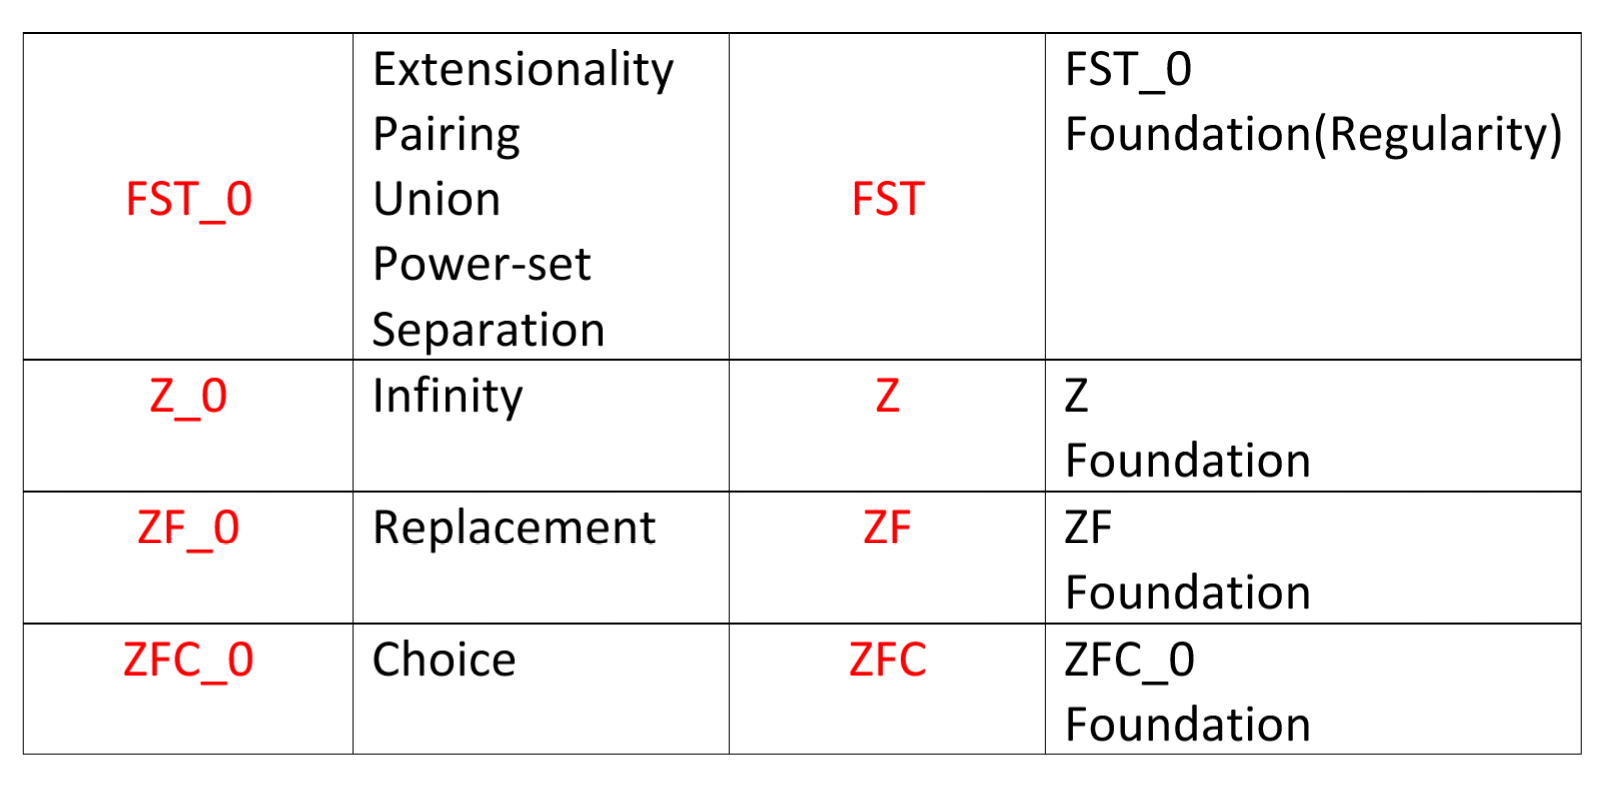
\includegraphics[scale=0.2]{1}
\end{center}
\end{figure}

What have we meant when we said set theory $T$? The notions differ from text to text, so here we will make a brief summary of different set axioms.
\s

The usual axioms are 1.Extensionality, 2.Pairing, 3.Union, 4.Power Set, 5.Separation(Aussonderung). These are all true in finite set systems, so we call them $\text{FST}_0$. (Finite Set Theory). If we add Foundation, we call it FST.

\quad If we add Infinity without Foundation(Regularity), we call it $Z_0$(Zarmelo). But what we usually call Zarmelo is $Z$, that has both Foundation and Infinity.

\quad If we add Replacement(Ersetzung) and Infinity in $\text{FST}_0$, we call it $ZF_0$, and $ZF$ if we have $ZF_0$ and foundation.

\quad $ZFC_0$ is $ZF_0$+Choice, and $ZFC$ is $ZFC_0$+Foundation.
\s

Note that, we have not considered the Empty Set Axiom.
\s

\subsubsection*{A long list of $\Delta_0^T$ formulas}

We say that an operation $x_1, \cdots, x_n \mapsto F(x_1, \cdots, x_n)$ is defined by a formula in class $\Gamma$ (where $\Gamma$ is any class of formulas) in the theory $T$ if there is a formula $\Psi \in \Gamma$ such that
\begin{align*}
&(1) \,\, T \proves \forall x_1, \cdots\forall x_n \exists y\,\, \Psi(x_1, \cdots, x_n, y)\\
&(2) \,\, T \proves \forall x_1, \cdots\forall x_n \forall y \forall z \,\, \Psi(x_1, \cdots, x_n, y) \wedge \Psi(x_1, \cdots, x_n,z) \rightarrow y=z \\
&(3) \,\, \Psi(x_1, \cdots, x_n, y) \quad \textit{iff} \quad y = F(x_1, \cdots, x_n)
\end{align*}
Note that point (3) is an informal requirement.
\s

\textbf{Examples :} $x\mapsto \{x\}$, $x,y \mapsto \{x,y\}$ \emph{[These are operations in $FST_0$!]}
\s

Now let us make a long list of $\Delta_0^T$ formulas for future use.

\begin{i}
\item[1.] $x\in y$
\item[2.] $x=y$. \quad 1 and 2 are both $\Delta_0$ without $T$.
\item[3.] $x\subset y$, is $\forall w(w\in x \rightarrow w\in y) \,\, \Leftrightarrow \,\,\forall w\in x(w\in y)$ so is $\Delta_0$ by definition ($T$ not needed)
\item[4.] $\Phi_0 (x) \,\, \Leftrightarrow \,\, \forall (w\not\in x) \,\, \Leftrightarrow \,\, \forall w(\neg w\in x) \,\, \Leftrightarrow \,\, \forall w(w\in x \rightarrow \neg x =x)$. This is $\Delta_0$ in predicate logic.
\item[5.] $x\mapsto \{x\}$. That is, $\Psi(x,z)$ defined by $\Psi(x,z)\,\, \Leftrightarrow \,\, ``z= \{x\}"$. Having this is equivalent to $\forall w (w\in z \leftrightarrow w=x) \,\, \Leftrightarrow \,\, \forall w(w\in z \rightarrow w=x)\wedge (w=x \rightarrow w\in z) \,\, \Leftrightarrow \,\, \exists w\in z(w=x) \wedge \forall w\in z (w\in z \rightarrow w=x)$ This is $\Delta_0$.
\item[6.] $x,y\mapsto \{x,y\}$.
\item[7.] $x.y\mapsto x\cup y$.
\item[8.] $x,y\mapsto x\cap y$.
\item[9.] $x,y\mapsto x\backslash y$.
\item[10.] $x,y \mapsto (x,y) = \{\{x\}, \{x,y\}\}$.
\end{i}
If two operations $f,g_1, \cdots, g_k$ are defined by $\Delta_0^T$ formulas, then so is the operation (\emph{Exercise})
\begin{align*}
x_1, \cdots, x_n \mapsto f(g_1(x_1, \cdots, x_n),\cdots, g_k(x_1, \cdots, x_n))
\end{align*}
We can extend the list using this fact.
\begin{i}
\item[11.] $x\mapsto x\cup \{x\} =: S(x)$ \emph{[By the previous fact, from 5 and 7.]}
\item[12.] $x\mapsto \cup x$.
\item[13.] the formula $\varphi$ describing ``$x$ is transitive".
\item[14.] the formula $\varphi$ describing ``$x$ is an ordered pair". \emph{[The quantifiers in this formula looks unbounded at the first glance, but we can use the fact that quantifies for the two component of $x$ are bounded by $\cup x$]}
\item[15.] $a,b \mapsto a\times b$ (Cartesian product)
\item[16.] The formula ``$x$ is a binary relation". \emph{[Similarly, the quantifiers look unbounded but is bounded under appropriate set of form $\cup x$.]}
\item[17.] $x\mapsto \text{dom}(x) := \{ y\,\, : \,\, \exists p \in x (p$ is an ordere pair, $p=(v,w)$ and $y=v\}$.
\item[18.] $x\mapsto \text{range}(x) := \{y : \exists p\in x(p$ is an ordered pair and $p=(v,y)) \}$.
\item[19.] the formula ``$v$ is a function".
\item[20.] the formula ``$x$ is injective".
\item[21.] the formula ``$x$ is a function from $A$ to $B$".
\item[22.] the formula ``$x$ is a surjection from $A$ to $B$". \emph{[it does not make sense to say that a function is a surjection without mentioning its range.]}
\item[23.] the formula ``$x$ is a bijection from $A$ to $B$". \emph{[note that, this indicates that the notion of being a bijection is the same in $A$ and $M$ - this is very important fact when we are working with continuum hypothesis in different models in that we want a bijective function to be a bijective function no matter in which level of the model we are working in.]}
\end{i}
\s

\subsubsection*{What is an ordinal?}

$\alpha$ is an \textbf{ordinal} if $\alpha$ is a \emph{transitive set, well-ordered by $\in$}.
\begin{subproof}
\emph{[Recall : what we mean by well ordered is that (1) is (strictly) totally ordered, (2) well-founded. (1) is a $\Delta_0$-formula. (2) can be written as $\forall x (\exists z\in x(\forall y\in x(\neg(y\in z)))$ which is a $\Pi_1$-formula, but not $\Delta_0^T$!]}

\quad We observe : \emph{``$(X,R)$ is a well-founded relation"} is not obviously absolute since the bound for the quantifier in
\begin{align*}
\forall z (z\subset X \rightarrow z \text{ has an }\epsilon\text{-minimal element})
\end{align*}
is the power set. (will be talking about absoluteness of well-foundedness on Friday.)

\quad But in models with the axiom of foundation, $\alpha $is an ordinal \emph{iff} $\alpha$ is transitive + totally ordred by $\epsilon$, \textit{i.e.} we do not have to worry about the existence of the $\epsilon$-minimality, so we do not have to worry about this problem anymore.
\end{subproof}
\s

\newday

(25th January, Friday)
\s

Last time : We made a list of things that are absolute for transitive models.

\quad Also we defined ``ordinals" : $x$ is an ordinal $\Leftrightarrow$ $\Phi_{ord}(x)$ $\Leftrightarrow$ $x$ is transitive and $(x, \epsilon)$ is a well-order (That is, $(x, \epsilon)$ is a total order and $\epsilon$ is a well-founded relation on $x$ (just $\Pi_1$)

\quad If $T$ contains the axiom of Foundation, then $\Phi_{ord}(x)$ $\Leftrightarrow$ $x$ is transitive and $(x,\epsilon)$ is a total order. This is also a $\Delta_0^T$ formula. Hence we can add some more itmes in our list of $\Delta_0^T$ formulas.

\begin{i}
\item[24.] ``$x$ is an ordinal" is $\Delta_0^T$ \emph{[for the right choice of $T$. So now we have the make track of which axiom system we are using - but of course in the lecture, we will often not mention this explicitly]}
\item[25.] ``$x$ is a successor ordinal" $\Leftrightarrow$ ``$x$ is an ordinal" + $\exists y\in x$ ($y$ is the $\epsilon$-largest element of $x$)
\item[26.] ``$x$ is a limit ordinal"
\item[27.] ``$x=\omega$" $\Leftrightarrow$ ``$x$ is the smallest limit ordinal". \emph{[Similarly we can talk about $x=\omega + \omega$, $x= \omega +1$, $x= \omega+\omega+1$, $x= \omega^2$, $x= \omega^3$, $\cdots$. This tells us that $\omega$ and related objects is uniquel existing in our model and is in the exactly right form we want them to be.]}
\end{i}
\s

\subsubsection*{Absoluteness of well-foundedness}

If $(X, R)$ is well-founded ($R$ the relation on $X$), we can define a \textbf{rank function}
\begin{align*}
\text{rk} : X \rightarrow \alpha, \quad \text{where } \alpha \text{ is some ordinal}
\end{align*}
such that $\text{rk}$ is order-preserving between $(X,R)$ and $(\alpha, \epsilon)$.
\begin{p}
: This theorem is proved using the right instance of Replacement. In particular, ZF proves that $(X, R)$ is well-founded $\Leftrightarrow$ $\exists \alpha \exists f (\alpha$ is an ordinal, $f$ is an order-preserving function from $(X, R)$ to $(\alpha, \epsilon)$.

\quad Thus for sufficiently strong $T$, ``$(X, R)$ is well-founded" is $\Delta_1^T$ and hence absolute for transitive models of $T$.
\end{p}
And we may generalise this to concepts defined by \textbf{transfinite recursion}.
\s

\defi We call the following a \textbf{Transfinite recursion theorem} : Let $(X,R)$ be wellfounded. Let $F$ be ``functional", so for every $x$ there is unique $y$ such that $y = F(x)$. Then there is a unique function $f$ with domain $X$ and for all $x\in X$,
\begin{align*}
f(x) = F(f | \text{IS}_R(x))
\end{align*}
where $\text{IS}_R(x) = \{ z\in X : zRx \}$.
\s

\prop Let $T$ be a set theory that is strong enough to prove the \emph{transfinite recursion theorem} for $F$. Let $F$ be absolute for transitive models of $T$ (\textit{i.e.} the formula defining $F$ is absolute). Let $(X, R)$ be in $A$ then $f$ defined by transfinite recursion is absolute between $A$ and $M$.
\begin{p}
: This is a generalisation of the result stated just above.
\end{p}
\s

This is a very important fact! For instance :
\s

\textbf{Example :} Let $L$ be any first order language whose symbols are all in $A$ (with $A$ strong enough). Then the set of $L$-formulas and the set of $L$-sentences are in $A$. The relation $S\models \varphi$ is defined by recursion and thus is absolute between $A$ and $M$.

\quad \emph{So} : if $S$ is an $L$-structure, $S\in A$, then 
\begin{align*}
(A, \epsilon) \models (S\models \varphi) \quad \Leftrightarrow \quad(M, \epsilon)\models (S\models \varphi)
\end{align*}
\s

Recall that,

\statement{G\"odel's incompleteness theorem} Let $T$ be a theory strong enough(\textit{e.g.} an arithmetic theory or a set theory). If $T$ is consistent, then $T \not\proves \text{Cons}(T)$ (\emph{\text{Cons}(T) is a sentence in $L$}).

\quad Exammples for such $T$ are : PA, Z, ZF, ZFC, $\zfc +\varphi$. In particular, this is also true for $\text{ZFC}^*$:=ZFC + Cons(ZFC) \emph{[hence ZFC* proves Cons(ZFC) but not Cons(ZFC*)]}
\s

By G\"odel's completeness theorem,
\begin{align*}
\text{Cons}(T) \quad \Leftrightarrow \quad \exists M (M \models T)
\end{align*} 
(Side fact : Cons(T) is $\Pi_1^Z$, and the RHS is $\Sigma_1^Z$, so in fact this shows $\Delta_0^Z$ for Cons($T$)!)
\s

\defi Write $\beta$ for ``there is a transitive set $A$ such that $(A, \epsilon) \models \zfc$". Clearly, $\beta$ implies Cons(ZFC).
\s

\thm If ZFC* is consistent, then ZFC*$\not\proves \beta$.
\begin{p}
\pf Let $(M, \epsilon) \models \zfc^*$. Suppose $\zfc^* \proves \beta$, so $(M, \epsilon) \models \beta$. Thus, in $M$, find $A$ transitive such that $(A, \epsilon) \models \zfc$. By assumption, $(M, \epsilon) \models \text{Cons(ZFC)}$. By G\"{o}del's completeness and absoluteness, $(A, \epsilon) \models \text{Cons}(ZFC)$. So putting these together, $(A, \epsilon) \models \zfc^*$.

\quad So we proved $\text{Cons(ZFC*)}$, Contradicting incompleteness theorem!

\eop
\end{p}
\s

That means that assuming $\beta$ is not an obvious assumption. so we need to study under which (natural) assumptions $\beta$ is true. So, let us investigate transitive models $A$ inside $M$.

\quad The two most basic constructions are the following :
\begin{i}
\item[(1)] \underline{von Neumann Hierarchy (cumulative hierarchy)}

Start with $V_0 := \phi$. Set $V_{\alpha+1} := \mathscr{P}(V_{\alpha})$ and $V_{\lambda} := \cup_{\alpha< \lambda} V_{\alpha}$ for a limit (ordinal) $\lambda$.
\s

\prop $\forall \alpha$, $V_{\alpha}$ is transitive. \emph{[prove by induction. key lemma : ``if $X$ is transitive, then $\mathscr{P}(X)$ is also transitive"]}

If $\lambda$ is a limit ordinal, then $V_{\lambda} \models \text{FST}$, If $\lambda > \omega$ and a limit, then $V_{\lambda}\models Z$.

\item[(2)] \underline{hereditarily small sets}

Let $\kappa$ be a cardinal. We say $X$ is hereditarily smaller than $\kappa$ if $|tcl(X)| < \kappa$ ($tcl$ is the transitive closure). Let $H_{\kappa} := \{X:X$ is hereditarily smaller than $\kappa \}$. Obviously transitive.
\end{i}
\s

\newday

(28th January, Monday)
\s

(The example sheet is already prepared - envelop next to C.0.10.).

\s
\subsubsection*{Concrete transitive models of ZFC :}

As in the last lecture, we consider the following two - by scruntinizing these two families models, we will find in which conditions the ZFC axioms can fail(in specific \emph{axiom of Replacement}), and therefore find an equivalent characterization of \emph{Replacement} given the rest axioms.
\begin{i}
\item[(1)] \underline{von Neumann Hierarchy (cumulative hierarchy)}, $V_{\alpha}$.

\item[(2)] \underline{hereditarily small sets}, $H_{\alpha}$.
\end{i}
We start with $V_{\alpha}$. We know : if $\lambda$ is a limit, $V_{\lambda} \models \text{FST}$, and if $h>w$, then $V_{\lambda} \models Z$. (see \emph{Example Sheet \#1}). Having this, we see that ZFC proves the consistency of Z - hence Z is critically weaker than ZFC. The critical axiom here is \emph{Replacement} and we do not want \emph{Replacement} to hold in von Neumann Hierarchy - if not, ZFC would prove the consistency of ZFC.

\quad Our test case would be $\lambda =\omega + \omega$. What does it mean for Replacement to fail? In our test case $V_{\omega + \omega}$, Replacement says :
\begin{align*}
& \text{If } F: V_{\omega + \omega} \rightarrow V_{\omega + \omega} \text{ is a definable function in } V_{\omega + \omega} \text{ and } x\in V_{\omega + \omega,}\\
& \text{then } \{F(y) : y\in x\} \in V_{\omega + \omega}.
\end{align*}
The idea is to take $x$ and $F$ so that this can not be true : take $x= \omega$ and
\begin{align*}
F : \begin{cases} 
u \mapsto \omega + u \quad \text{if } u\in \omega\\
y\mapsto 0 \quad \text{if } y\not\in \omega
\end{cases}
\end{align*}

\begin{figure}[h]
\begin{center}
    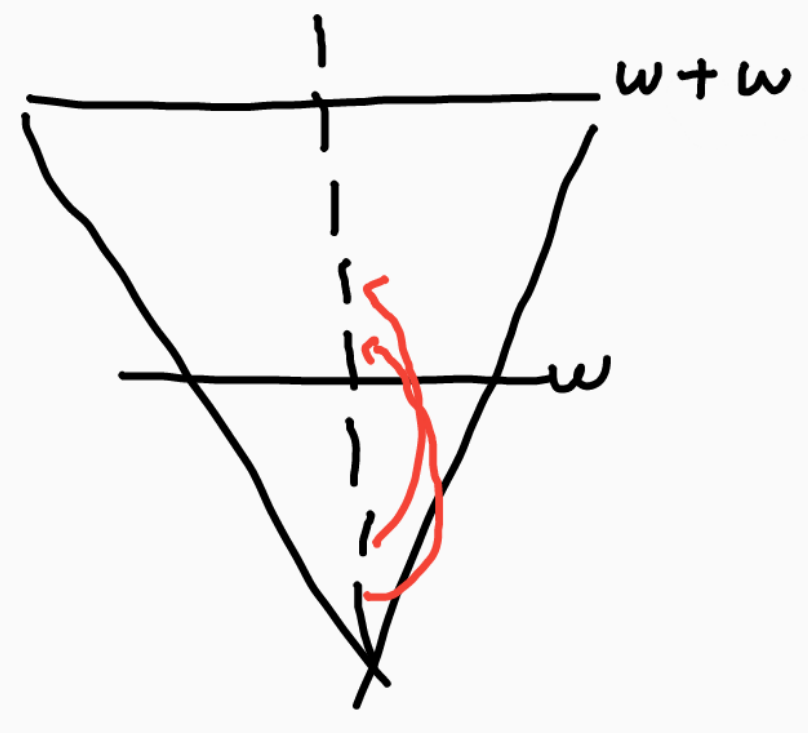
\includegraphics[scale=0.25]{2}
\end{center}
\end{figure}

Let $Y = \{F(n): n\in \omega\}$. Then $Y\in V_{\omega+\omega +1} \backslash V_{\omega + \omega}$. This example shows concretely that $V_{\omega+\omega} \models \neg \text{Replacement}$.
\s

\quad Let us think why our example failed. Similarly as for $\omega + \omega$, if $\alpha$ is an ordinal such that there is a definable function $f: \omega \rightarrow \alpha$ such that the range of $f$ is unbounded in $\alpha$ then $V_{\alpha} \models \neg \text{Replacement}$. Even more geenrally, if $\beta < \alpha$ and a definalbe function $f: \beta \rightarrow \alpha $ with unbounded range, then $V_{\alpha} \models \neg \text{Replacement}$.
\s

To avoid this problem, we now turn our attention to the hereditary small sets. Recall,

\defi We call a cardinal $\kappa$ \textbf{regular} if there is no partition
\begin{align*}
\kappa = \bigcup_{i\in I} A_i
\end{align*}
such that $|I|, |A_i| <\kappa$ for all $i\in I$. \emph{[Equivalently, for every $\alpha < \kappa$ there is no unbounded function $f: \alpha \rightarrow \kappa$ - this seems to be the right definition that can avoid the problem suggested above]}.

\quad We know, for example, that $\aleph_1$ is regular. Moreover, for any $\alpha$, $\aleph_{\alpha +1}$ is regular.
\s

\quad So our next candidate for the model would be $\alpha = \aleph_{1}$. Here, $\mathscr{P}(\omega) \in V_{\omega +2} \subset V_{\omega_1}$. Clearly, by the definition of $\omega_1$ (recall, $\omega_1$ is defined to the the smallest ordinal such that $\omega$ does not surject in. Also by diagonal argument, $\mathscr{P}(\omega)$ does not surject in $\omega$) there is a surjection
\begin{align*}
s: \mathscr{P}(\omega) \rightarrow \omega_1
\end{align*}
so the range of $s$ is unbounded in $\omega_1$. Thus : $V_{\omega_1} \models \neg \text{Replacement}$.

\begin{figure}[h]
\begin{center}
    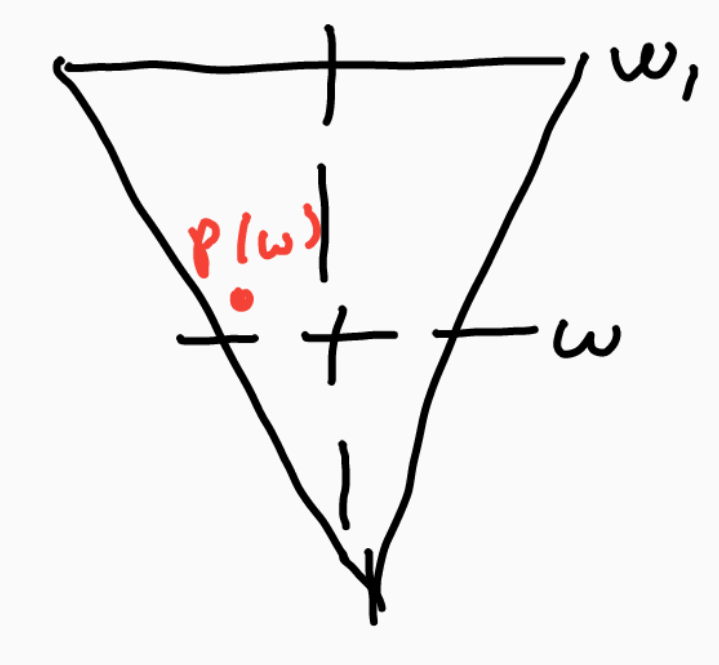
\includegraphics[scale=0.25]{3}
\end{center}
\end{figure}

\quad In general, if $\kappa$ is regular and there is $\lambda < \kappa$ with $|\mathscr{P}(\lambda)|\geq \kappa$, then the same argument shows $V_{\kappa} \models \neg \text{Replacement}$.
\s

Having these, now it seems that it is necessary to make additional hypothesis to make a model of our theory.
\s

\defi A cardinal $\kappa$ is called \textbf{inaccessible} if
\begin{i}
\item[(a)] $\kappa$ is regular.
\item[(b)] $\forall \lambda > \kappa$, $|\mathscr{P}(\lambda)| < \kappa$, \quad \textbf{[Strong Limit]}
\end{i}
The most basic example for this is the natural numbers. We want to see if there is a different example for this.
\s

\emph{[Side note : Related to the question, we may ask ``Are there regular limit cardinals?". Under GCH (generalized continuum hypothesis, $\forall \kappa,2^{\kappa} = \kappa^+$), we have : $\kappa$ is accesible $\Leftrightarrow$ $\kappa$ is regular limit. So we already see that this question is not easy to answer. This property is called \textbf{weak inaccessibility}, and in fact can not be proved with current axiom system.]}
\s

\emph{[A short history from Wikipedia page, ``Inaccessible cardinal : The term "inaccessible cardinal" is ambiguous. Until about 1950 it meant "weakly inaccessible cardinal", but since then it usually means "strongly inaccessible cardinal". An uncountable cardinal is weakly inaccessible if it is a regular weak limit cardinal. It is strongly inaccessible, or just inaccessible, if it is a regular strong limit cardinal (this is equivalent to the definition given above). Some authors do not require weakly and strongly inaccessible cardinals to be uncountable (in which case $\aleph_{0}$ is strongly inaccessible). Weakly inaccessible cardinals were introduced by Hausdorff (1908), and strongly inaccessible ones by Sierpi\'nski \& Tarski (1930) and Zermelo (1930)."]}
\s

Let us assume that $\kappa> \omega$ is inaccessible. 
\s

\lem $\forall \lambda < \kappa$, $|V_{\lambda}|< \kappa$.
\begin{p}
\pf Clealy $|V_{\omega}| = \aleph_{0}$, so $|V_{\omega}| < \kappa$.

\quad We prove by induction - suppose $|V_{\lambda}| < \kappa$. Then $V_{\lambda +1}= \mathscr{P}(V_{\lambda})$, so $|V_{\lambda +1}| = |\mathscr{P}(V_{\lambda})|< \kappa$ by (b) in the previous definition. Now let $\lambda < \kappa$ be a limit ordinal. Then $V_{\lambda} = \bigcup_{\alpha < \lambda} V_{\alpha}$. Suppose for a contradiction that $|V_{\lambda}| = \kappa$. But $|V_{\alpha}| < \kappa$ for all $\alpha < \kappa$, so you can write $\kappa$ as a union of $\lambda$ many things of smaller cardinality. this contradicts regularity.

\eop
\end{p}
\s

In the example of $V_{\omega_1}$ above, Replacement failed because $V_{\omega + 2}$ was too big in $V_{\omega_1}$. This will not happen given the assumption of inaccessibility.
\s

\thm If $\kappa$ is inaccessible, then $V_{\kappa} \models \text{Replacement}$.
\begin{p}
\pf

\quad Take any $F:V_{\kappa} \rightarrow V_{\kappa;}$ and any $x\in V_{\kappa} =\bigcup_{\alpha < \kappa}V_{\alpha}$. Thus, find $\alpha \in \kappa$ such that $x\in V_{\alpha}$. Since $V_{\alpha}$ is transitive, $x\subset V_{\alpha}$, so $|x| \leq |V_{\alpha}| < \kappa$ (by lemma).

\quad Now consider $X:=\{F(y) : y\in x\}$. For each $y\in x$, consider the 
\begin{align*}
&\rho(F(y)) :=\text{least } \alpha \text{ such that }F(y) \in V_{\alpha +1}\backslash V_{\alpha}\\
& R:= \{ \rho(F(y)) : y\in x\}
\end{align*}
Note that we can define $R$ because by accessibility, $\rho(F(y))< \kappa$. We also have $|R| \leq |x|< \kappa$. Hence regularity, $\beta := \cup R < \kappa$. This tells us that $\forall y\in x$, $F(y)\in V_{\beta +1}$. So $X\subset V_{\beta+1}$, $X\in V_{\beta+2}$. This provides Replacement.

\eop 
\end{p}
\s

This also shows that existence of inaccessible sets can not be proved in ZFC.
\s

\newday

(30th January, Wednesday)
\s

\textbf{Last lecture :} we had the notion of inaccessible cardinal. Write \textbf{IC} for the axiom ``there is an inaccessible cardinal". If $\kappa$ is inaccessible, then $V_{\kappa} \models \text{ZF}$ (in particular, the Replacement). In fact, $V_{\kappa} \models \zfc$ (not very dfficult to check Choice, as $V_{\kappa}$ is a transitive model). So
\begin{align*}
\zfc + \text{IC} \proves \text{``there is a transitive set that is a model of ZFC"} (=: \beta)
\end{align*}
So We had proved that ZFC+Cons(ZFC)$\not\models \beta$, so ZFC+Cons(ZFC)$\not\models$IC.
\s

It is also convincing that weak accessibility does not contradict ZFC, but nobody actually succeeded for 110 years.
\s

\subsubsection*{Two model-theoretic reminders}
\begin{i}
\item[(1)] \emph{L\"owenheim-Skolem theorem} : If $S$ is any structure in some countable first-order language $L$ and $X\subset S$ is any subset, then there is a \textbf{Skolem hull} of $X$ in $S$, $X\subset \mathcal{H}^S(X) \subset S$ such that
\begin{i}
\item[(a)] $\mathcal{H}^S(X) \prec S$ (elementary substructure of $S$), \textit{i.e.} 
\begin{align*}
\forall \varphi \forall h_1,\cdots,h_n \in \mathcal{H}^S(X)\quad \mathcal{H}^S(X) \models \varphi(h_1, \cdots, h_n) \,\, \Leftrightarrow \,\, S\models \varphi(h_1, \cdots, h_n).
\end{align*}
\item[(b)] $|\mathcal{H}^S(X)| \leq \max (\aleph_0, |X|)$.
\end{i}
\begin{subproof}
\textbf{proof sketch)} Key ingredient is to use Tarski-Vaught criterion
\begin{subproof}
: $Z\subset S$ then $Z\prec S$ \emph{iff} for every $\varphi$ and all $z_1, \cdots, z_n$, if $S\models \exists x\,\, \varphi(x, z_1, \cdots,z_n)$, then $Z\models \exists x\,\, \varphi(x, z_1, \cdots, z_n)$
\end{subproof}

Then let $Z_0 := X$, and inductively define
\begin{align*}
&Z_1 := X\cup\text{the witness for all tuples }\varphi, z_1, \cdots, z_n\text{ where }z_1, \cdots, z_n \in Z_0,\\
&Z_{n+1} :=Z_n \cup\text{the witness for all tuples }\varphi, z_1, \cdots, z_n\text{ where }z_1, \cdots, z_n \in Z_0 \quad \text{ and}\\
&Z := \cup_{n\in \mathbb{Z}}Z_n.
\end{align*}
Then $Z$ is as desired.
\end{subproof}
\emph{Consequence} : If we work in model $(M, \epsilon) \models \text{ZFC+IC}$, we can find inaccessible $\kappa$ with $V_{\kappa} \models \zfc$, and $V_{\kappa} \subset M$. Apply L\"owenheim-Skolem to $V_{\kappa}$ with $X:= \phi$, then $H:= \mathcal{H}^{V_{\kappa}} (\phi) \prec V_{\kappa}$, so $H\models \zfc$. The cardinality of $\mathcal{H}^{V_{\kappa}} (\phi)$ is $\leq \aleph_0$, so we found a countable model of ZFC.

\quad Then By construction, $\aleph_1 \in H$.
\begin{subproof}
: There is a formula $\varphi$ such that $\varphi(x)$ \emph{iff} $x$ is the least uncountable cardinal. In ZFC, $V_{\kappa} \models \exists x\,\, \varphi(x)$ but the only element that satisfies $\varphi$ in $V_{\kappa}$ is $\aleph_1$. So in the Skolem hull construction, $\aleph_1 \in Z_1 \subset H$
\end{subproof}

This implies that $H$ can not be transitive, since $\aleph_1$ has uncountable many element, but $H$ has only countably many element.
\s

\item[(2)] \emph{Mostowski Collapse Theorem} : If $X$ is any set and $R\subset X\times X$ such that $R$ is well-defined and extensional, then there is a transitive set $T$ such that
\begin{align*}
(T, \epsilon) \cong (X, R)
\end{align*}
Consider $(H, \epsilon) \models \zfc$ (\textit{e.g.} constructed by L\"owenheim-Skolem as above). Since $(H, \epsilon) \models \zfc$, $\epsilon$ is extensional on $H$. Since $\epsilon$ (in $M$) is well-founded, $\epsilon$ is well-founded on $H$. So let $T$ be the Mostowski collapse of $H$. $T$ is transitive, so
\begin{align*}
(T, \epsilon) \cong (H, \epsilon)
\end{align*}
By this isomorphism, $(T, \epsilon) \models \zfc$, and since this is a bijection, $|T| = |H| \leq \aleph_0$. Together, there is a countable transitive model of ZFC.
\end{i}
This fact is very important : if we are working in ``the universe of set", we have no potential to manipulate, because we can not add any set in it! But if we are working in a countable transitive model, it is small enough that there are various manipulations available.
\s

\begin{figure}[h]
\begin{center}
    \begin{subfigure}[b]{0.3\textwidth}
        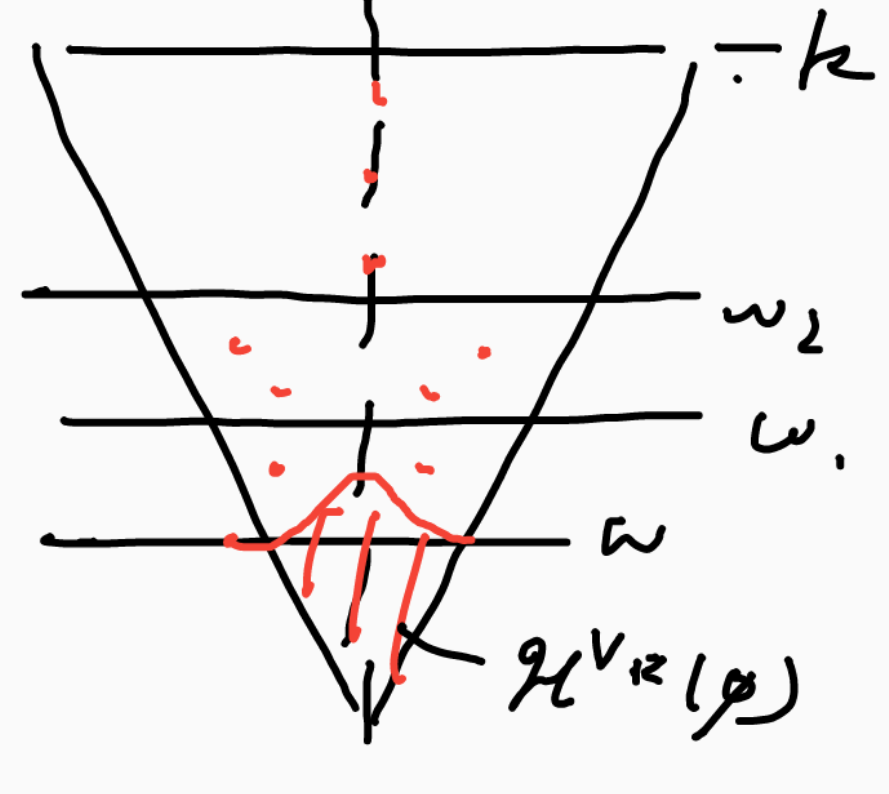
\includegraphics[scale=0.16]{4}
    \end{subfigure}
    \begin{subfigure}[b]{0.3\textwidth}
        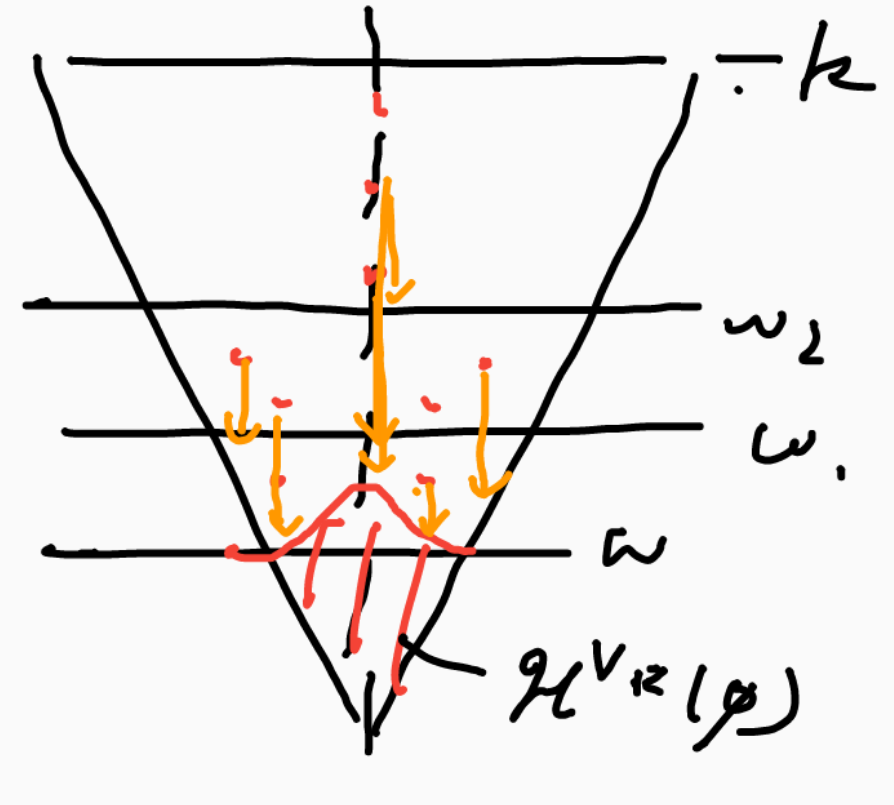
\includegraphics[scale=0.16]{5}
    \end{subfigure}
    \begin{subfigure}[b]{0.3\textwidth}
        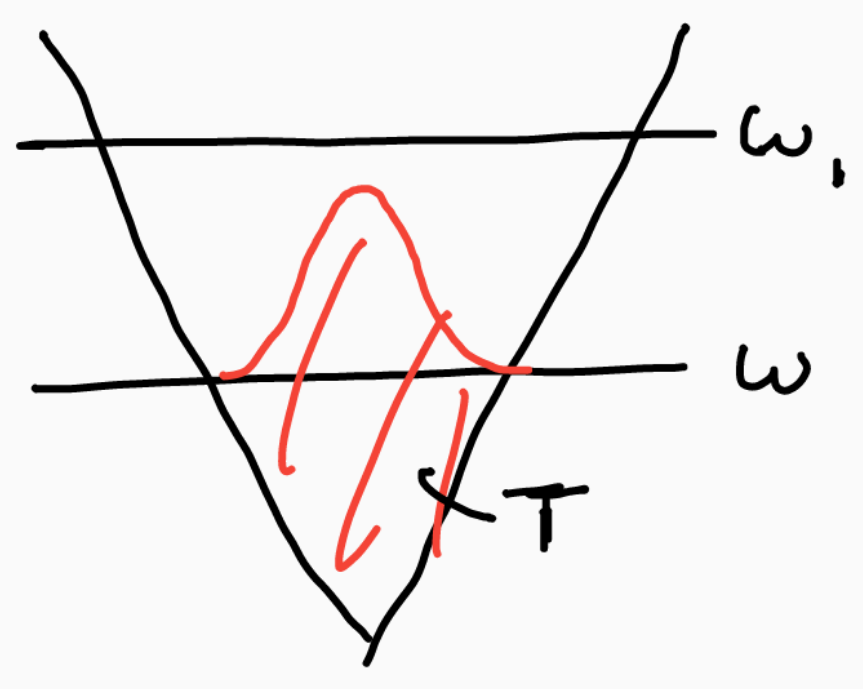
\includegraphics[scale=0.19]{6}
    \end{subfigure}
\end{center}
\end{figure}

Now let us think about some formulas that could test absoluteness of models just constructed.
\begin{itemize}
\item Consider $\varphi(x) := x\text{ is countable}$ $\Leftrightarrow$ $\exists f(f: x\rightarrow \mathbb{N}, f \text{ is injective})$. Each component is $\Delta_0^{\zfc}$, so $\varphi$ is a $\Sigma_1^{\zfc}$ formula, so \emph{upwards absolute}.

\quad But this formula is \emph{not downwards absolute}
\begin{subproof}
: If $\alpha \in \text{Ord}$, $\alpha \in T$, then $V_{\kappa} \models \alpha$ is countable. But since $(T, \epsilon) \models \zfc$, there is some $\alpha \in T$ such that $(T, \epsilon) \models \alpha$ is uncountable, so $V_{\kappa}$ and $T$ disagree about the truth value of $\varphi(\alpha)$.
\end{subproof}

\item Conversely, consider $\psi(x) := x \text{ is a cardinal}$ $\Leftrightarrow$ $\forall \alpha (\alpha < x \rightarrow \text{there is no injection from } x \text{ to } \alpha)$. This is in $\Pi_1^{\zfc}$ so \emph{downwards absolute}. In $(T, \epsilon)$, take $\alpha$ least such that $(T, \epsilon) \models \psi(\alpha)$. Then $(T, \epsilon) \models \alpha$ is a cardinal. Clearly, $V_{\kappa} \models \alpha$ is not a cardinal, so $\psi$ is \emph{not upwards absolute}.
\s

Note that if $\lambda$ is an countable cardinal in $V_{\kappa}$, then $\lambda \not\in T$, so the downwards absoluteness of $\psi$ is not very interesting. Hence instead of building $\mathcal{H}^{V_{\kappa}}(\phi)$, build $H^* := \mathcal{H}^{V_{\kappa}}(\omega_1 +1)$. Clearly $\omega_1 \in H^*$ and $\omega_1 \subset H^*$, so $\omega_1 \subset T^*$ and $\omega_1 \in T^*$. So $|H^*| = \aleph_1$. 

\begin{figure}[h]
\begin{center}
    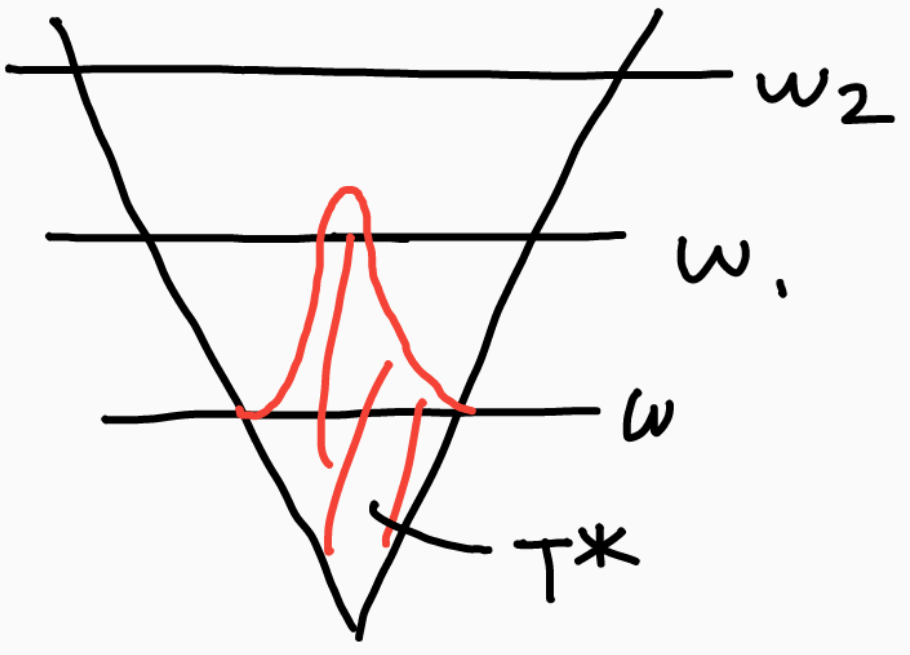
\includegraphics[scale=0.25]{7}
\end{center}
\end{figure}

Now we have $V_{\kappa} \models (\omega_1 \text{ is a cardinal}"$ is downwards absolute, and so $T^* \models (\omega_1 \text{ is a cardinal})$. 
\end{itemize}
\s

\newday

(1st February, Friday)
\s

\emph{What have done so far} : 1. Decided to go for transitive models, 2. Looked at ``inner models". 3. In particular, models of type $V_{\alpha}$. 4. Seen : if $\alpha$ is inaccessible, then $V_{\alpha} \models \zfc$. 5. Found countable transitive submodels $T \subset V_{\alpha}$ such that $T\models \zfc$, by using L\"owenheim-Skolem and Mostowski collaption.
\s

Seems good so far, but$\ldots$

\emph{One problem} : this is \emph{not} going to change the truth value of CH.
\begin{subproof}
: Suppose CH is true in $(M, \epsilon)$, so there is a bijection between $\reals$ (or just $\mathscr{P}(\mathbb{N}))$ and $\omega_1$. But all the objects we use are all in $V_{\kappa}$ for reasonably large $\kappa$, so $(M, \epsilon) \models$CH $\Leftrightarrow$ $(V_{\kappa}, \epsilon) \models$CH. By L\"owenheim-Skolem, we got countable $H \prec V_{\kappa}$ so $(H, \epsilon) \models$CH is equivalent to $(V_{\kappa}, \epsilon)\models$CH. And Mostowski gets $(T, \epsilon) \cong (H, \epsilon)$, so $(T, \epsilon)\models$CH $\Leftrightarrow$ $(H, \epsilon) \models$CH.
\end{subproof}
\s

\textbf{Summary :} The method of finding countable transitive \emph{elementary} submodels of $V_{\kappa}$ is not going to change the value of CH. So we need a different construction.
\s

\subsubsection*{The second construction : models of hereditarily small sets.}

\defi Let $\kappa$ be a regular cardinal, \textit{e.g.} $\kappa =\omega$, or $\omega_1$. Then $x$ is called \textbf{hereditarily of size less than $\kappa$} if $|\text{tcl}(x)|< \kappa$.

\quad The class of all such functions is designated $H_{\kappa}$.
\s

Recall, $\text{tcl}(x)$ is defined as $\bigcup_{n\in \mathbb{N}} t_n(x)$, where $t_0(x)=x$ and $t_{n+1} (x) = \cup t_n(x)$. The definition of $\text{tcl}(x)$ captures the intuition of \emph{``$x$ has size $< \kappa$, all elements have size $\kappa$, all elements of element of $x$ have size $<\kappa$, etc."}.
\s

\emph{[Side remark : if $\kappa$ is not regular, this intuition might not work : let $\kappa = \aleph_{\omega}$. Then define
\begin{align*}
x^0_{n} = \aleph_{n}, \quad x^{k+1} = \{x_n^k \}, \quad X = \{x_0^0, x_1^1, x_2^2, x_3^3, \cdots \}
\end{align*}
Then $X$ is countable. In the transitive closure notation above, $|t_{n+1}(X)|= \aleph_n$. But $|\text{tcl}(X)|= \aleph_{\omega}$.]}
\s

\textbf{Useful Observations :}
\begin{i}
\item[1.] $H_{\kappa}$ is transitive.
\item[2.] If $X\subset H_{\kappa}$ and $|X| <\kappa$, then $X\in H_{\kappa}$ - this follows directly from regularity of $\kappa$ and the definitions.
\end{i}
\s

\textbf{$\clubsuit$ First example :} $H_{\aleph_0} =: HF$ (Hereditarily finite)
\begin{subproof}
\textbf{Claim :} $HF = V_{\omega}$
\begin{subproof}
\pf To see $V_{\omega} \subset HF$, we need to show $V_n \subset HF$ for all $n$. Clearly, $V_0 =\phi\subset HF$. If $V_n \subset HF$ and $Z\subset V_n$, then by \textbf{Observation 1 and 2}, $Z\in HF$, so $\mathscr{P}(V_n) = V_{n+1}\subset HF$.

\quad To see $HF \subset V_{\omega}$, prove by contradiction - suppose not, so there is $x\in HF\backslash V_{\omega}$. Take such an $x$ with minimal rank $\alpha$. Then $x\in V_{\alpha +1} \backslash V_{\alpha}$. In particular, $V_{\alpha} \subset HF$. Hence $x\in \mathscr{P}(V_{\alpha})$, so $x\subset V_{\alpha} \subset H$, $x\in HF$, so $x$ is finite (note, if $y\in HF$ with $\rho(y) < \alpha$, then there is $k\in \mathbb{N}$ such that $\rho(y)=k$). Write $x=\{x_1, \cdots, x_n\}$. By minimality, each of them is in $V_{k_i}$ for some $k_i$. So $x\in V_{\max(k_1, \cdots, k_n)+1} \subset V_{\omega}$, which is a contradiction.
\end{subproof}
\end{subproof}
\s

\textbf{$\clubsuit$ Second example :} $H_{\aleph_1} =: HC$ (Hereditarily countable)
\begin{subproof}
We have $\text{Ord} \cap HC = \omega_1$, $V_{\omega +2} \backslash HC \neq \phi$ and $V_{\omega+1}\subset HC$.

\quad Which axioms are true in $HC$?
\begin{subproof}
\textbf{Pair :} $x,y\in HC$. Then $\{x,y\} \subset HC$ and $|\{x,y\}| < \aleph_1$, so $\{x,y\}\in HC$.

\quad Separation, Foundation, Extensionality, Union, all hold in $HC$ without much doubt. Ones worth discussing are Replacement and Power set.
\s

\textbf{Replacement :} Let $F: HC \rightarrow HC$ and $x\in HC$. Consider the range $R:= \{F(y) : y\in x\}$. Then, $|R| \leq |x| < \aleph_1$ and $R\subset HC$, and therefore by Observation 2, $R\in HC$. So Replacement follows without much work.
\s

\textbf{Power set :} The Power set is the most problematic one. We know that $\mathbb{N} \in HC$, while $\mathscr{P}(\mathbb{N}) \not\in HC$. This is in fact \emph{not} enough to show $HC \models \neg$Power-set. Instead, we need to show that for all $A\in HC$,
\begin{align*}
HC\models ``A\text{ is not the power set of }\mathbb{N}" \,\, \Leftrightarrow \,\, \exists X(X\subset \mathbb{N} \wedge X\not\in A)
\end{align*}
Thus suppose, for all $X$, $X\subset \mathbb{N}$ and $X\in HC$ implies $X\in A$. But if $X\subset \mathbb{N}$, then $X\subset HC$ and $|X| < \aleph_1$ so $X\in HC$. So if $A$ is any set such that $\forall X(X\subset \mathbb{N} \text{ and } X\in HC \rightarrow X\in A)$ then $A$ is uncountable, so $A\not\in HC$. Therefore,
\begin{align*}
HC \models \neg \text{Power-set}
\end{align*}  
\end{subproof}
\end{subproof}
\s

\newday

(4th February, Monday)
\s

\textbf{Recall :} $H_{\kappa}$ was a model of all of ZFC without power set if $\kappa$ is regular.
\s

\prop If $\kappa$ is a \emph{strong limit}, then $H_{\kappa} \models \text{Power-set}$.
\begin{p}
\pf We will show that : if $x\in H_{\kappa}$, then $\mathscr{P}(x) \in H_{\kappa}$. [This is much stronger than the Power set axiom.] Let us look at
\begin{align*}
\text{tcl}(\mathscr{P}(x)) = \mathscr{P}(x) \cup \text{tcl}(x)
\end{align*}
but $\mathscr{P}(x)$ has size $2^{|x|}< \kappa$ and $\text{tcl}(x)$ has size $< \kappa$, so together $\text{tcl}(\mathscr{P}(x))$ has size $<\kappa$, so $\mathscr{P}(x) \in H_k$

\eop
\end{p} 
\s

However, in fact, you will see in \emph{Example sheet \# 1} that for $\kappa$ inaccessible, $H_{\kappa}$ and $V_{\kappa}$ are identical, so we can not say anything more interesting in this setting. So for a genuine outbreak, we need a different idea.
\s

\emph{General idea :} Build inner models using ``definability" properties.
\s

But the problem is that Definability is not definable :
\s

\thm \emph{(Tarski, undefinability of truth)} \emph{[This is bit funny, because Tarski was actually the one who defined what the truth is.]} (We will only think about the set theory setting here, but has more general notion of undefinability)

\quad Let $(M, \epsilon) \models \zfc$. We assume that the language of set theory $\mathscr{L}_{\epsilon} \subset M$. Consider the sets
\begin{align*}
&S \text{ of sentence of } \mathscr{L}_{\epsilon}, \quad \textit{and} \\
&U \text{ of every predicates} (\mathscr{L}_{\epsilon} \text{-formulas in one free variable})
\end{align*}
A truth predicate would be a formula $T(x)$ in $\mathscr{L}_{\epsilon}$, i.e. $T\in U$, such that
\begin{align*}
(M, \epsilon) \models \varphi \quad \Leftrightarrow \quad (M, \epsilon) \models T(\varphi)
\end{align*}
Then there can be no such truth predicate. That is, there is no thing that can be viewed as a truth `internally'.

\quad \emph{[Contrast with our previous result : $\text{If } M \text{ is a set, then } (M, \epsilon) \models \varphi \text{ is } \Delta_0$]}
\begin{p}
\pf \emph{(Idea : diagonalisation)} If $\varphi(x) \in U$, then we can ask whether $\varphi(\varphi)$ is true (note $\varphi(\varphi) \in S$).

\quad Let's assume that $T$ is a truth predicate, and define $\delta(x) := \neg T(x(x))$ where $x(x)$ is $x$ applied to $x$ if $x$ is a predicate($x\in U$) and is $\phi$ if otherwise, \textit{i.e.} the ``diagonal". Now apply $\delta$ to $\delta$, so $\delta(\delta) \in S$. Then
\begin{align*}
M \models \delta(\delta) \quad &\Leftrightarrow \quad M \models T(\delta(\delta)) \quad \text{ since } T \text{ was a truth predicate} \\
&\Leftrightarrow \quad  M \models \neg T(\delta(\delta)) \quad \text{by definition of } \delta
\end{align*}
which is a contradiction.

\eop
\end{p}
\s

\defi Again, let $M\models \zfc$. We say that $x\in M$ is \textbf{definable} if there is a formula $\varphi$ such that 
\begin{align*}
\forall y\in M, \quad x=y \,\, \Leftrightarrow \,\, M\models \varphi(y)
\end{align*}
We say that a formula $D$ is called a \textbf{definition of definability if} $\forall x\in M$,
\begin{align*}
x \text{ is definable} \,\, \Leftrightarrow \,\, M \models D(x)
\end{align*}
\s

\thm \emph{(Undefinability of Definability)} There is no formula $D$ that is a definition of definability.

\quad \emph{[again, the problem is that we have to define what definability is from `inside'. From outside, it is easy to define definability - just make the definition above to a formula]}
\begin{p}
\pf Assume that $D$ is a definition of definability. Consider
\begin{align*}
\alpha := \min \{ \beta\,\, : \,\, \beta \text{ is not definable but } \forall \gamma < \beta, \exists \gamma'(\gamma < \gamma'< \beta \text{ and } \gamma' \text{ is definable}) \},
\end{align*}
the supremum of the definable ordinals (can do the same for the least definable object, but the formula is slightly more complicated). This is defined by the formula
\begin{align*}
y=\alpha \leftrightarrow  \text{ is an ordinal and } \neg D(y) \text{ and } \forall \gamma (\gamma < y \rightarrow \exists \gamma' (\gamma < \gamma' < y \wedge D(\gamma'))) 
\end{align*}
This proves that $\alpha$ is definable, so
\begin{align*}
M \models D(\alpha)
\end{align*}
But one of the conjunctions in the definition implies $M\models \neg D(\alpha)$, a contradiction!

\eop
\end{p}
\s

Recall, our general idea was to build inner models using ``definability" properties. We now learned that ``definability" is not going to work without keeping track of parameters. So, we need to define ``definability" with direct reference to what parameters are allowed.
\s

\defi Fix $A$ and $n\in \mathbb{N}$. We are going to define by recursion what it means to be \textbf{definable subset of $A^n$} :
\begin{align*}
\text{Diag}_{\epsilon}(A, n, i,j) = &\{ s\in A^n : s_i \in s_j \}\\
\text{Diag}_{=}(A, n, i,j) = &\{ s\in A^n : s_i = s_j \}\\
\text{Proj}(A, R,n) = &\{ s\in A^n : \exists t\in R (t \upharpoonright n = s) \}, \quad R\subset A^{n+1} \text{ and } t \upharpoonright n \text{ the projection onto } n \text{ conjunctions}\\
\text{Def}(0, A, n) = &\{ \text{Diag}_{\epsilon}(A, n, i,j) : i,j < n\} \cup \{\text{Diag}_{=}(A, n, i,j) : i,j<n \} \\
\text{Def}(k+1, A, n) = & \,\text{Def}(k, A, n) \cup \{R\cap S : R,S\in \text{Def}(k, A, n)\} \\
&\cup \{ A^n \backslash S : S\in \text{Def}(k, A, n) \} \cup \{ \text{Proj}(A, R,n) : R\in \text{Def}(k, A, n+1) \} \\
\text{Def}(A,n) = &\bigcup_{k\in \mathbb{N}} \text{Def}(k, A, n)
\end{align*}
\s

\textbf{Observe :} The definition of $\text{Defi}(k+1, A,n)$ and $\text{Defi}(0, A,n)$ is $\Delta_0$, so the definition of of $\text{Defi}(A,n)$ is a recursive definition based on absolute notions and thus absolute for transitive models (containing $A$).

\emph{[this construction works better then the previous one, since everything is bounded by $A^n$]}
\s

\textbf{Next thing :} Use $\text{Def}(A, n)$ to define the ``definable power set". After that, define a ``definable von Neumann hierarchy".
\s

\newday

(6th February, Wednesday)
\s

\subsubsection*{The constructible universe}

We were on construction of an inner model $L\subset M$ that is based on definability.

\textbf{Problems with definability} : connected to \emph{Tarski's undefinability proof}. The ``definable" fragment of truth is that whether we fix the scope of existential quantifiers in advance. 

\quad So we recursively defined $\text{Def}(A, n)$ - the definable subsets of $A^n$ where ``definable" is interpreted in $A$.
\s

\lemnum{1} If $X\subset A^n$ is such that there is a formula $\varphi$ such that
\begin{align*}
(x_1, \cdots, x_n) \in X \quad \Leftrightarrow \quad (A, \epsilon) \models \varphi(x_1, \cdots, x_n)
\end{align*}
Then $X\in \text{Def}(A,n)$.
\begin{p}
\pf Simple (but lengthy) induction over complexity of $\varphi$.
\end{p}
\s

\lemnum{2} In $M$, we have that $\text{Def}(A,n)$ is countable. \emph{[We even have a concrete surjection $\mathbb{N}\rightarrow \textnormal{Def}(A,n)$]}
\begin{p}
\pf Direct from the definition.
\end{p}

\textbf{Observe :} In the definition of $\text{Def}(k, A, n)$, we only used notions absolute for transitive models of ZF. So, since $\text{Def}(A, n)$ was defined by recursion over $\text{Def}(k, A,n)$, also $\text{Def}(A,n)$ is absolute between transitive models. (So different models will agree on what is definable in this sense.)
\s

\textbf{Goal :} to see Definable power set

$\text{Def}(A, 1)$ would be the easiest choice, but it is not a good candidate - if $A$ is uncountable, then there is $a\in A$ such that $\{a\} \not\in \text{Def}(A, 1)$ by \textbf{Lemma 2}.
\s

\defi We define the \textbf{definable power set} by
\begin{align*}
\mathscr{D}(A) := \{X\subset A : \exists n \, \exists s \in A^n \, \exists R\in \text{Def}(A,n+1)\,\,\text{such that } X= \{a \in A : (a, s_0, \cdots, s_{n-1}) \in R \}\}
\end{align*}
\s

\textbf{Observe 1:} If $X$ is informally definable with parameters from $A$, \textit{i.e.} $X= \{a\in A : (A, \in) \models \varphi(a, p_1, \cdots, p_n) \} \text{ for some } p_1, \cdots, p_n \in A$ then $X\in \mathscr{D}(A)$,
\s

\textbf{Observe 2:} As $\text{Def}(A,n)$ was absolute and the quantifiers in the definition of $\mathscr{D}(A)$ are all bounded, $\mathscr{D}(A)$ is absolute for transitive models.
\s

\prop If $A$ is transitive, then $\mathscr{D}(A)$ is transitive.
\begin{p}
\pf Suppose $x\in X \in \mathscr{D}(A)$. Then has $x\in X \subset A$, and by transitivity of $A$, has $x\subset A$. But since also $x \in A$, we can define $x$ as a subset by the formula $\varphi(x) := (v\in x)$, so
\begin{align*}
x = \{z\in A : (A, \in) \models \varphi(z) \}
\end{align*}  
\eop
\end{p}
\s

\subsubsection*{Constructible hierarchy}

\defi Take \begin{align*}
L_0 &:= \phi \\
L_{\alpha+1} &:= \mathscr{D}(L_{\alpha}) \\
L_{\lambda} &:= \bigcup_{\alpha < \lambda} L_{\alpha}
\end{align*}
We refer to the class $\bigcup_{\alpha \in \text{ord}} L_{\alpha}$ as ``$L$" or \textbf{``the constructible universe"}.
\s

\textbf{Properties}
\begin{i}
\item[(1)] If $\alpha \leq \omega$, then $V_{\alpha} = L_{\alpha}$
\item[(2)] For every $\alpha$, $L_{\alpha}$ is transitive [Follows from Proposition by induction]
\item[(3)] $\alpha \leq \beta$ $\rightarrow$ $L_{\alpha} \subset L_{\beta}$
\item[(4)] $\text{Ord} \cap L_{\alpha} = \alpha$. (see (3), (4) in the second example sheet)
\item[(5)] If $\alpha \geq \omega$, then $|L_{\alpha}| = |\alpha|$.
\begin{subproof}
\pf Prove by induction. For $\alpha = \omega$, have $|L_{\omega}| = |V_{\omega}| = \aleph_0 = |\omega|$. Suppose for all $\beta < \alpha$ we have $|L_{\beta} |\leq |\beta|$. Will show that $|L_{\alpha}| < |\alpha|^+$. 
\begin{i}
\item[-] Case 1 : if $\alpha$ is a successor, say $\alpha = \beta +1$, has $L_{\alpha} = L_{\beta+1} = \mathscr{D}(L_{\beta})$. Then there is a surjection from $\aleph_0 \times \bigcup_{n\in \mathbb{N}}L_{\beta}^n$ onto $\mathscr{D}(L_{\beta})$, as $\aleph_0 \times \bigcup_{n\in \mathbb{N}}L_{\beta}^n$ has cardinality $|L_{\beta}|$.
\item[-] Case 2 : if $\alpha$ is a limit, let $\pi_{\beta} : \alpha \rightarrow L_{\beta}$ be a surjection. Then we find surjection $\alpha\times \alpha \rightarrow L_{\alpha}, (\gamma, \gamma') \mapsto \pi_{\gamma}(\gamma')$.

\eop
\end{i}
\end{subproof}
\end{i}
\s

What is the relation between $V_{\omega +1}$ and $L_{\omega +1}$? We have $L_{\omega+1} \subset V_{\omega+1}$ but $V_{\omega +1} \backslash L_{\omega +1} \neq \phi$, since $V_{\omega +1}$ is uncountable while $L_{\omega +1}$ is countable.

\begin{figure}[h]
\begin{center}
    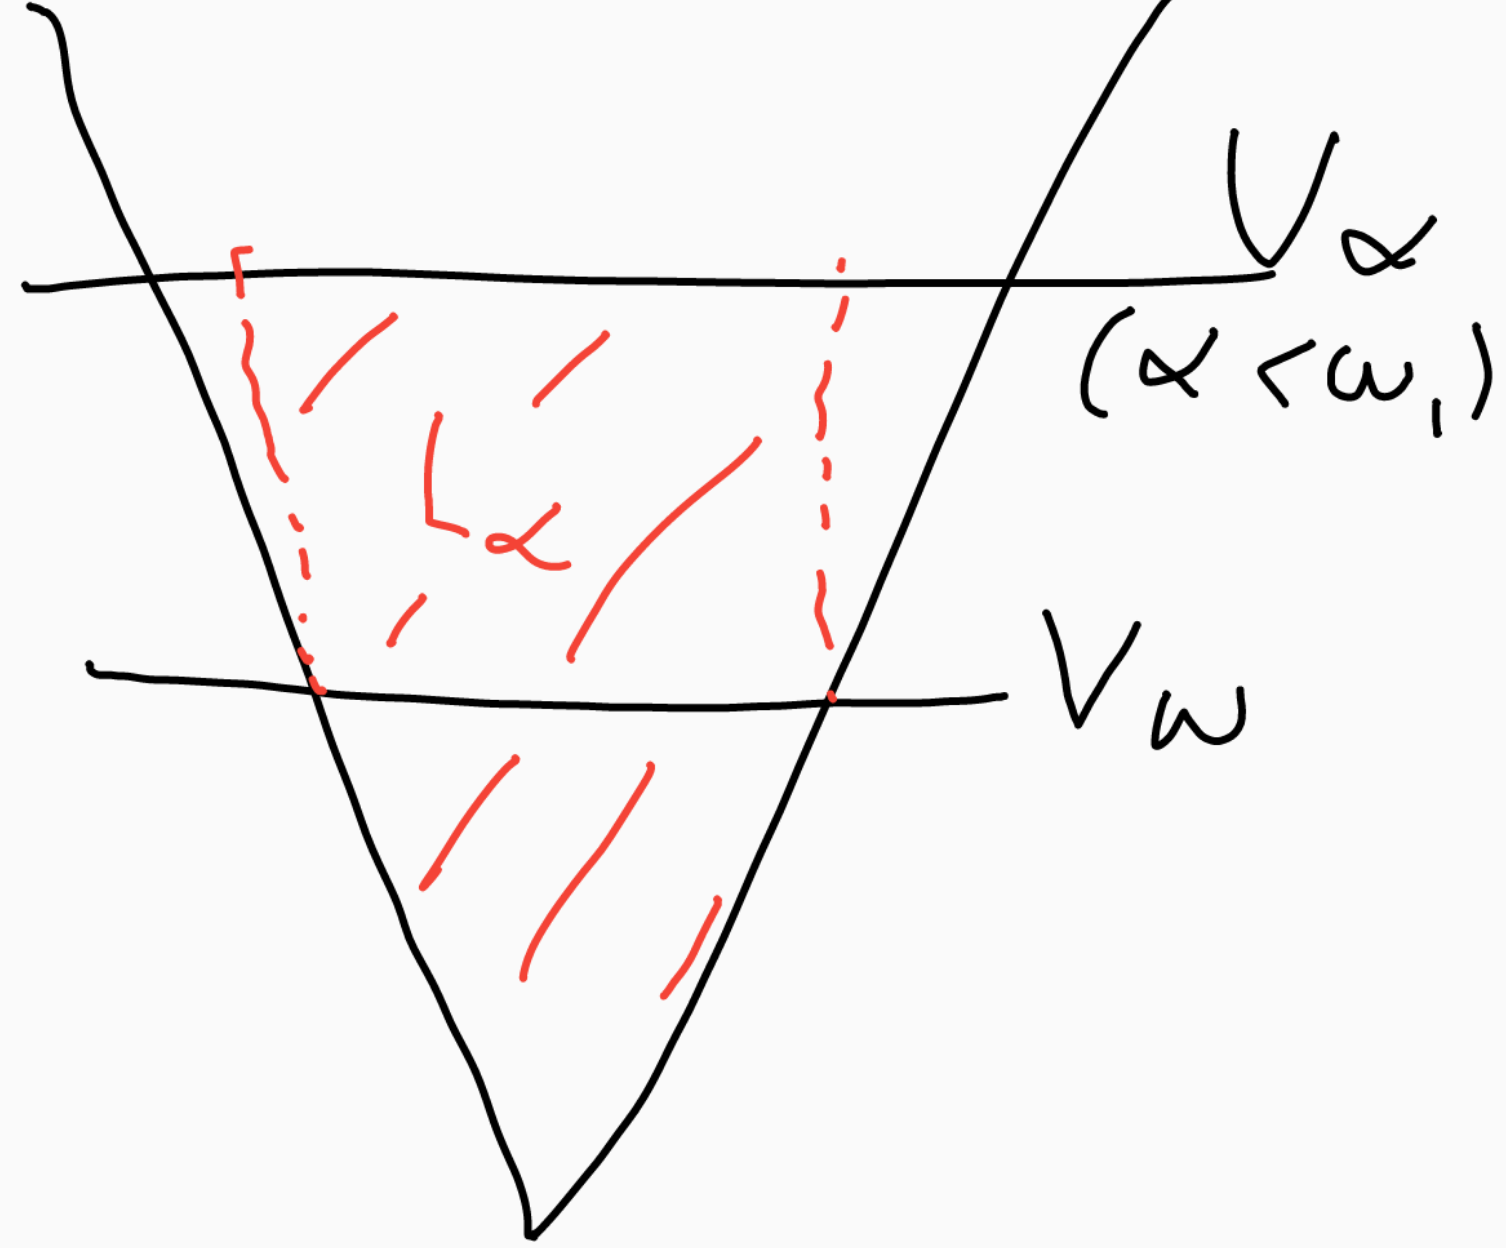
\includegraphics[scale=0.13]{8}
\end{center}
\end{figure}

\quad The question whether the picture of $L_{\alpha}$ in $V_{\alpha}$ really captures the right object is really crucial for us.
\s

\defi If $x$ is constructible, $x\in L$, then define
\begin{align*}
\rho_L(x) := \min \{\alpha : x\in L_{\alpha +1}\}
\end{align*}
The crucial point about relationship between $V_{\omega +1}$ and $L_{\omega +1}$ is encoded in this object.
\s

\defi $V=L$ is the \textbf{Axiom of Constructibility},
\begin{align*}
\forall x \exists \alpha (x\in L_{\alpha})
\end{align*}
\s

\lem If $M$ is a transitive set model of $\zfc + (V=L)$, then there is a limit ordinal $\lambda$ such that $M= L_{\lambda}$.
\begin{p}
\pf Consider $\lambda := \text{Ord} \cap M$ (note this is a limit ordinal - if it is a successor, then it is the largest ordinal, which is refutable in ZFC). We claim that $M = L_{\lambda}$.

\quad Suppose $x\in M$, by $(V=L)$, we may find $\alpha \in M$ such that $(M, \epsilon) \models x\in L_{\alpha}$. $L_{\alpha}$ was defined by recursion from absolute notions, so $x\in L_{\alpha}$ is absolute, hence $x\in L_{\alpha} \subset L_{\lambda}$. So $M \subset L_{\lambda}$.

\quad Suppose $x\in L_{\lambda}$, so there is $\alpha < \lambda$ such that $x\in L_{\alpha}$, so $(M, \epsilon) \models(x\in L_{\alpha})$. So by choice of $\lambda$, has $x\in M$.

\eop
\end{p}
\s

\newday

(8th February, Friday)
\s

Recall, we had the constructible universe $L_{\lambda}$.
\s

\defi We let $\Phi(x, \alpha)$ the formula describing ``$x\in L_{\alpha}$" and $\Psi(x,\alpha)$ the formula describing ``$x=L_{\alpha}$". Then both $\Psi$ and $\Phi$ are absolute for transitive models of set theory.
\s

We were proving,

\prop If $A$ is a transitive set model of $\zfc + (V=L)$, then $A=L_{\alpha}$ where $\alpha = \text{Ord} \cap A$.
\begin{p}
\pf The first direction ``$A\subset L_{\alpha}$" : if $x\in A$, then by $(A, \epsilon)\models (V=L)$, find $\beta$ such that $(A, \epsilon) \models (x\in L_{\beta})$ and by absoluteness, $x\in L_{\beta} \subset L_{\alpha}$.

\quad ``$L_{\alpha} \subset A$" : Suppose $x\in L_{\alpha}$. Since $\alpha =\text{Ord} \cap A$ and $A\models \zfc$, $\alpha$ has to be a limit ordinal. Then $L_{\alpha}$ is, by definition, $L_{\alpha} = \bigcup_{\beta < \alpha} L_{\beta}$, so may find $\beta < \alpha$ and $x\in L_{\beta}$. Since $(A, \epsilon) \models \zfc$, we know that $A$ thinks ``$L_{\beta}$ exists" (formally, there is $X$ such that $(A, \epsilon) \models \Psi(X, \beta)$). By absoluteness of $\Psi$, we have $\Psi(X, \beta)$, so $X= L_{\beta}$. Therefore $L_{\beta} \in A$, and since $x\in L_{\beta}$, by transitivity of $A$, has $x\in A$.

\eop
\end{p}
\s

This proposition is only useful when a model of $\zfc + (V=L)$ exists. So our next major goal is :
\s

\thm \emph{(G\"odel, 1938)} If $\kappa$ is inaccessible, then $L_{\kappa}\models \zfc+ (V=L)$. 
\s

Assuming this theorem, we have a quite unexpected result :
\s

\corr If $\kappa$ is inaccessible, then there is a countable $\alpha$ such that $L_{\alpha} \models\zfc + (V=L)$.
\begin{p}
\pf Take $H:= \mathcal{H}^{L_{\kappa}}(\phi) \prec L_{\kappa}$. Then $H$ is countable. Take $T\cong H$, the Mostowski collapse. Then $(T, \epsilon) \equiv (L_{\kappa}, \epsilon)$ and is countable, transitive. In particular, $(T, \epsilon) \models \zfc + (V=L)$.

\quad By previous proposition, $T= L_{\alpha}$ for some ordinal $\alpha$. By one of the properties of $L$, we have $|L_{\alpha}| = |\alpha|$, so $\alpha$ is countable.

\eop 
\end{p}
\s

\textbf{Contrast this with :} if $V_{\alpha} \models \zfc$, then $\alpha$ can not be countable. If $\alpha$ is countable, there is a code for a surjection $f: \mathbb{N} \rightarrow \alpha$ in $V_{\omega+1} \subset V_{\alpha}$, so $V_{\alpha}\models ``\alpha$ is countable", a contradiction to $V_{\alpha} \models \zfc$ (in particular a contradiction to \textbf{Power-set}). 
\s

\begin{p}
\textbf{proof of G\"odel's theorem)} We check each axiom.

\quad \textbf{Extensionality :} follows from the transitivity. 

\quad \textbf{Pair :} $x,y\in L_{\kappa}$, find $\alpha$ such that $x, y\in L_{\alpha}$, $\{x,y\}\subset L_{\alpha}$. Clearly, the formula $\varphi(z, x,y) := (z=x\vee z=y)$ define the pair $\{x,y\}$ so by a previous observation (\textbf{Observation 1} of last lecture), the pair lives in $\mathscr{D}(L_{\alpha})=L_{\alpha+1} \subset L_{\kappa}$ (in fact, this is not the exact statement that of \textbf{Observation 1} from last lecture - it only states that $\{x,y\}$ is in $\mathscr{D}(A)$ viewed from outside (or so called $M$), not $L_{\kappa}$. This proof only worked, because $\varphi$ was quantifier-free, hence can be interpreted in exactly the same way in different models.)

\quad The same proof takes care of, say, \textbf{Union} - because the defining formula is absolute.

\quad \textbf{Power-set :} Consider $x\in L_{\kappa}$. As before, take $\alpha < \kappa$, $x\in L_{\alpha}$. $L_{\alpha}$ is transitive so $x\subset L_{\alpha}$, and so $|x|\leq |L_{\alpha}| < \kappa$, because $\kappa$ was strongly inaccessible.

\quad Consider $\mathscr{P}(x)$ in $M$ (the set system), then $|\mathscr{P}(x)| =2^{|x|} < \kappa$, again because $\kappa$ was inaccessible. Then $|L_{\kappa} \cap \mathscr{P}(x)| \leq |\mathscr{P}(x)| < \kappa$. \emph{[Caution : Since $L_{\kappa}$, $\mathscr{P}(x)$ are sets in $M$, $L_{\kappa} \cap \mathscr{P}(x)$ is a set in $V_{\kappa}$ and it is definable in $V_{\kappa}$ by the formula $z\in L_{\kappa}\cap \mathscr{P}(x)$ $\Leftrightarrow$ $\Phi(z, L_{\kappa})\wedge z\subset x$ But that's not good enough to prove that $L_{\kappa} \cap \mathscr{P}(x) \in L_{\kappa}$]} For each $z\in L_{\kappa} \cap \mathscr{P}(x)$, find $\alpha_z := \rho_L(z) < \kappa$. Consider $\{\alpha_z : z\in L_{\kappa}\cap \mathscr{P}(x) \} \subset \kappa$ - this is of size $<\kappa$. By the regularity of $\kappa$, find a bound $\beta < \kappa$ such that $\{ \alpha_z : z\in L_{\kappa} \cap \mathscr{P}(x) \} \subset \beta$. So $L_{\kappa} \cap \mathscr{P}(x) \subset L_{\beta}$. Define
\begin{align*}
P:= \{z: (L_{\beta}, \in) \models z\subset x\}
\end{align*}
By our observation (from last lecture), $P\in \mathscr{D}(L_{\beta}) = L_{\beta+1} \subset L_{\kappa}$. But $L_{\kappa} \models \forall z(z\in P \Leftrightarrow z\subset x)$ so $L_{\kappa}$ is a model of the \textbf{Power-set axiom}. \emph{[The critical thing about this proof is that the actual power set of $x$ may not be the power set that $L_{\kappa}$ thinks - we only picked up the subsets of $x$ that are definable in $L_{\kappa}$.]}
\end{p}
\s

\newday

(11th February, Monday)
\s

(Example sheet \#2 in envelope next to C0.10)
\s

We were proving,

\thm If $\kappa$ is inaccessible, then $L_{\kappa} \models \zfc + (V=L)$.
\begin{p}
\textbf{proof continued)} We saw \textbf{Pairing} and \textbf{Power-set}.
\s

\textbf{Separation :} Let $x\in L_{\kappa}$, $\varphi$ be a formula, $a_1, \cdots, a_n \in L_{\kappa}$. Separation says that $\{z\in x : \varphi(z, a_1, \cdots, a_n) \}$ exists. More formally, $\{ z\in x : L_{\kappa} \models \varphi(z, a_1, \cdots, a_n) \}$.

\quad For each $1\leq i\leq n$, find $\alpha_i < \kappa$ such that $a_i \in L_{\alpha_i}$, find $\alpha < \kappa$ such that $x\in L_{\alpha}$. Define $\beta := \max \{ \alpha, \alpha_1, \cdots, \alpha_n \}$. So for any $z\in x$, we have $z, a_1, \cdots, a_n \in L_{\beta}$, by transitivity of $L_{\beta}$. So $\{ z\in  x : L_{\beta} \models \varphi(z, a_1, \cdots, a_n) \} \in \mathscr{D}(L_{\beta}) = L_{\beta+1}$.

\quad \emph{But the problem is : in proving Power-set, the formula was absolute between $L_{\beta}$ and $L_{\kappa}$ so that we could just transfer this to $L_{\kappa}$. However, in this setting, we have $\{ z \in x: L_{\beta} \models \varphi(z, a_1, \cdots, a_n) \} \neq \{ z\in x : L_{\kappa}\models \varphi(z, a_1, \cdots, a_n) \}$  for general $\varphi$, so we can not apply the same method.}

\quad Instead, we consider $\mathcal{H}^{L_{\kappa}}(L_{\beta}) \prec L_{\kappa}$ with $|\mathcal{H}^{L_{\kappa}}(L_{\beta})| = |L_{\beta}| = |\beta| < \kappa$. Now consider its \emph{Mostowski collapse}, $T \cong \mathcal{H}^{L_{\kappa}}(L_{\beta})$ with Mostowski isomorphism $\pi : T \rightarrow \mathcal{H}^{L_{\kappa}}(L_{\beta})$. Here $T$ is transitive, and $|T| = |\mathcal{H}^{L_{\kappa}}(L_{\beta})| < \kappa$.

(Recall, from model theory, $M\cong M'$ means $M\models \varphi (x_1, \cdots, x_n)$ $\Leftrightarrow$ $M' \models \varphi(\pi (x_1), \cdots, \pi(x_n)))$.

\quad $M\equiv M'$ means $M\models \varphi$ $\Leftrightarrow M'(\varphi)$ for $\varphi$ sentence. So $M \cong M'$ implies $M \equiv M'$.

\quad $M\prec M'$ means $M\models \varphi(x_1, \cdots, x_n)$ $\leftrightarrow$ $M' \models \varphi(x_1, \cdots, x_n)$.)

We get
\begin{align*}
\begin{array}{ccccc}
T & \xrightarrow{\pi} & \mathcal{H}^{L_{\kappa}}(L_{\beta}) & \xrightarrow{id} & L_{\kappa} \\
\varphi(z, a_1, \cdots, a_n) & \mapsto & \varphi(\pi(z), \pi(a_1), \cdots, \pi(a_n)) & \mapsto & \varphi(\pi(z), \pi(a_1), \cdots, \pi(a_n))
\end{array}
\end{align*}
We know that the Mostowski collapse is the identity on transitive sets. So if $X\subset L_{\kappa}$ is transitive, then $\pi \upharpoonright X = id \upharpoonright X$. Since $L_{\beta}$ is transitive and all $z, a_1, \cdots, a_n$ are in $L_{\beta}$,
\begin{align*}
T\models \varphi(z, a_1, \cdots, a_n) \quad \Leftrightarrow \quad L_{\kappa} \models \varphi(z, a_1, \cdots, a_n)
\end{align*}
Let's do the ``modified Skolem hall construction" from \emph{Example \#12 of Example Sheet \#1} : take
\begin{align*}
\alpha_0 =& \text{Ord} \cap T\\
\alpha_{n+1} &\text{ is the last } \gamma \text{ such that } L_{\gamma} \text{ contains } L_{\alpha_n} \\
&\text{ and a witness for each existential statement true with parameters in } L_{\alpha_n} \\
\bar{\alpha} =& \bigcup_{n\in \mathbb{N}}\alpha_n
\end{align*} 
then $T\prec L_{\bar{\alpha}}$ with $\bar{\alpha} < \kappa$. Define the set via $\varphi$ over $L_{\bar{\alpha}}$ :
\begin{align*}
& \{z\in x: L_{\bar{\alpha}} \models \varphi(z, a_1, \cdots, a_n) \} = \{z\in x : T\models \varphi(z, a_1, \cdots, a_n) \} \\
=& \Big\{ z\in x : \mathcal{H}^{L_{\kappa}} (L_{\beta}) \models \varphi(\pi(x), \pi(a_1), \cdots, \pi(a_n)) \Big\} \\
=& \{ z\in x : \mathcal{H}^{L_{\kappa}}(L_{\beta}) \models \varphi(x, a_1, \cdots, a_n))\} \\
=& \{z\in x: L_{\kappa} \models \varphi(z, a_1, \cdots, a_n) \} 
\end{align*}
but we have $\{z\in x: L_{\bar{\alpha}} \models \varphi(z, a_1, \cdots, a_n) \} \in \mathscr{D}(L_{\bar{\alpha}}) = L_{\bar{\alpha}+1}$.

\quad Hence we showed Pair, Power-set, Separation. The rest is similar - do as an exercise.

\eop
\end{p}
\s

\thm \emph{(The Condensation Lemma)} If $\kappa$ is inaccessible, $x, y\in L_{\kappa}$, $y\subset x$, then there is $\alpha < \kappa$ with $|\alpha| \leq |\text{tcl}(x)|$ such that $y\in L_{\alpha}$.
\begin{p}
\pf Consider $y\subset x$ and $\text{tcl}(x\cup \{y\}) =:t$. Clearly, $|t| = |\text{tcl}(x)|$. Consider Mostowski collapse of Skolem hull,
\begin{align*}
T \xrightarrow{\pi} \mathcal{H}^{L_{\kappa}}(t) \prec L_{\kappa}
\end{align*}
so $|T| = |\mathcal{H}^{L_{\kappa}}(t)| = |t| = |\text{tcl}(x)|$. $\pi$ is the identity on $t$ (as $t$ is transitive), so $\pi(y)=y$ and $\forall z\in x$, $\pi(z) =z$, $\pi(x)=x$.

\quad By the first proposition of last lecture, we may find $\beta$ such that $T=L_{\beta}$ \emph{[Now we are allowed to do this, since $L_{\kappa} \models \zfc +(V=L)$ and therefore $L_{\beta} \equiv L_{\kappa} \models \zfc+(V=L)$]}. Now $y$ can be defined over $L_{\beta}$ with parameters in $L_{\beta}$. Also has $|\mathcal{H}^{L_{\kappa}}(t)| = |t| = |\text{tcl}(x)| = |L_{\beta}|= |\beta|$, so $\beta$ has the right size.

\eop
\end{p}
\s

\newday

(13th February, Wednesday)
\s

We are going to prove consistency of CH today!! Goal : There is a model of $\zfc + \ch$.
\s

Recall, we had

\textbf{Condensation lemma)} Let $\kappa$ be inaccessible. For $x, y\in L_{\kappa}$ and $y\subset x$, there is $\alpha$ such that $|\alpha| \leq |\text{tcl}(x)|$ and $y\in L_{\alpha}$.
\s

\emph{[Recall, a one-line proof of the Condensation lemma : we have
\begin{align*}
y \in L_{\alpha} = T \cong \mathcal{H}^{L_{\kappa}}(\text{tcl}(x) \cup \{y\}) \prec L_{\kappa}
\end{align*}
]}
\s

\corrnum{1} If $x= \mathbb{N}$, $y\subset \mathbb{N}$, then there is $\alpha < \omega_1$ such that $y\in L_{\alpha}$.
\s

\corrnum{2}
\begin{i}
\item[1.] $\mathscr{P}(\mathbb{N}) \cap L_{\kappa} \subset L_{\omega_1}$. Observe that $\mathscr{P}(\mathbb{N}) \cap L_{\kappa} = \mathscr{P}^{L_{\kappa}} (\mathbb{N})$ where $\mathscr{P}^{L_{\kappa}} (\mathbb{N})$ refers to the unique $p\in L_{\kappa}$ such that $L_{\kappa} \models (p = \mathscr{P}(\mathbb{N}))$.
\item[2.] $\mathscr{P}^{L_{\kappa}} (\mathbb{N}) \subset L_{\omega_1}$.
\item[3.] $|\mathscr{P}^{L_{\kappa}} (\mathbb{N})| \leq |L_{\omega_1}| = |\omega_1| = \aleph_1$.
\end{i}
\s

Let us improve this to show $L_{\kappa} \models CH$.

\textbf{Key idea} : $L_{\kappa} \models \zfc$, the Condensation Lemma is a theorem of ZFC, so apply CL inside $L_{\kappa}$. But the problem is : in fact our Condensation lemma is a theorem of ZFC + IC.
\s

\emph{Remark :} so if you assume ZFC + 2IC (that is, there are at least two inaccessible cardinals.) in $M$, then this argument gets you that $L_{\kappa} \models CH$ for $\kappa$ the second inaccessible. \emph{[This feels a bit odd. Let's try to do this without the second inaccessible]}
\s

Work in $L_{\kappa}$. We know that $\mathscr{P}^{L_{\kappa}}(\mathbb{N}) \subset L_{\omega_1}$ where $\omega_1$ is the $\omega_1$ in $M$. Note that $\omega_1 < \kappa$, $L_{\omega_1}\subset L_{\kappa}$. So we have, for some $\beta$,
\begin{align*}
\mathscr{P}^{L_{\kappa}}(\mathbb{N}) \subset L_{\beta} =T \cong \mathcal{H}^{L_{\kappa}}(L_{\omega_1}) \prec L_{\kappa}
\end{align*}
By the standard argument, we get $\beta < \aleph_2 < \kappa$. But now $L_{\beta} \models \zfc + (V=L)$. Run the CH proof for $V_{\kappa}$ as $M$ and $L_{\beta}$ as $L_{\kappa}$ :
\begin{align*}
y \in L_{\alpha} = T \cong \mathcal{H}^{L_{\beta}}(\mathbb{N}\cup \{y\}) \prec L_{\beta}
\end{align*}
Now $L_{\kappa} \models ``\alpha \text{ is countable"}$. So if $\omega_1^{L_{\kappa}}$ is the $\omega_1$ of $L_{\kappa}$, then $\mathscr{P}^{L_{\kappa}}(\mathbb{N}) \subset L_{\omega_1^{L_{\kappa}}}$ so $L_{\kappa} \models 2^{\aleph_0} \leq \aleph_1$. Hence $L_{\kappa} \models CH$.
\s

\thm $\text{Cons(ZFC + IC)} \Rightarrow \text{Cons(ZFC + CH)}$.
\s

\emph{Comments :}
\begin{itemize}
\item[1.] The same argument with $x= \lambda$ for some $L_{\kappa}$-cardinal $\lambda$ gives us $L_{\kappa} \models 2^{\lambda} \leq \lambda^+$. So GCH(generalized continuum hypothesis) holds : for all $\lambda$, $2^{\lambda} = \lambda^+$.
\item[2.] What about the inaccessible condition? Can we remove IC?
\begin{itemize}
\item[(a)] If we have transitive set model of ZFC, we can mimic this proof. But this is still a stronger assumption than just ZFC.
\item[(b)] There is a way of getting around assumption (a) as well : Use the Le\'vy Reflection Theorem (see \emph{Example Sheet \#2}) : fix in advance some finite list $\Phi$ of sentences you wish to preserve and find sufficiently large $\alpha$ such that $\Phi$ is absolute for $V_{\alpha}$. 

\quad Go through all needed absoluteness results and lemmas and theorems and collect for each of them $\varphi$ the finite set $\Phi_{\varphi}$ of axioms of ZFC needed to prove them. Form $\Phi := \bigcup_{\varphi \text{ is relevent}} \Phi_{\varphi}$ noting that relevant $\varphi$ are finite.

\quad Apply \emph{L\'evy Reflection Theorem} to $\Phi$ and run the previous proof to get a model of $\Phi + \ch$. Now consider all finite subset $\Psi$ such that $\Phi \subset \Psi \subset \zfc$ and get models of $\Psi + \ch$. Then compactness gives a model of $\zfc + \ch$.
\end{itemize}
\item[3.] Consider $L = \bigcup_{\alpha \in \text{ord}} L_{\alpha} \subset M$. Our proof does not say what axioms hold in $L$, but using the \emph{L\'evy Reflection Theorem}, you can prove that if $V\models \zfc$, then $L \models \zfc + (V=L)$.
\end{itemize}
\s

\textbf{The question about regular limit cardinals} : we studied the notions of regular/singular, successor/limit and have seen
\begin{center}
\begin{tabular}{ c c c }
{} & Regular & Singular \\
Successor & O & X \\
Limit & $?$ & O
\end{tabular}
\end{center}
If we strengthen ``limit"($\forall \lambda< \kappa(\lambda^+< \kappa)$) to ``strong limit"($\forall \lambda< \kappa (2^{\lambda}  < \kappa)$), then we showed that ZFC cannot prove the (existence of regular strong limits) = (Existence of inaccessible cardinals) where $\mathscr{P}^{L_{\kappa}}(\mathbb{N})$ refers. 
\s

Clearly ZFC+GCH$\rightarrow$(every limit is a strong limit). So ZFC+GCH$\rightarrow$(every regular limit is an inaccessible cardinal) $\cdots (\star)$.
\s

We have : $\zfc \not\proves$(there are regular limits)
\begin{p}
\pf Assume that $M\models \zfc$ and that $\zfc \proves \text{(there are regular limits)}$. Towards a contradiction (with G\"odel), prove $M\models \cons(\zfc)$.

\quad Consider $L\subset M$, then by \textbf{Comment 3}, $L\models \zfc + \text{GCH}$. By $\zfc \proves \exists \text{regular limit}$, has $L \models \zfc + \text{GCH} +\exists \kappa (\kappa\text{ is regular limit})$, and so by ($\star$), has $L\models \zfc + \text{IC}$. This gives $L \models \exists \kappa (L_{\kappa} \models \zfc)$, so $L\models \cons(\zfc)$, which concludes $M\models \cons(\zfc)$ - a contradiction with G\"odel.

\eop
\end{p}
\s

\newday

(18th February, Monday)
\s

\subsection*{The limitation of the method of inner models}

\defi If $(M, \in) \models \zfc$, $N\subset M$, we say that $N$ is an \textbf{inner model of M} if
\begin{i}
\item[(a)] $(N, \in) \models \zfc$,
\item[(b)] $\text{Ord} \cap N = \text{Ord} \cap M$,
\item[(c)] $N$ is transitive in $M$.
\end{i}
\s

\thm \emph{(Minimality Theorem)} If $M \models \zfc + (V=L)$ and $N$ is an inner model of $M$, then $N=M$. \emph{[That is, we do not have proper inner model (in a sense).]}
\begin{p}
\pf We know that $M = \bigcup_{\alpha \in \text{Ord} \cap M} L_{\alpha}^M$ where $L_{\alpha}^M$ is the set $L_{\alpha}$ (interpreted in $M$). This follows directly from $V=L$ in $M$. So in order to show $N = M$, it is enough to show that $L^M_{\alpha} \subset N$ for all $\alpha \in \text{Ord} \cap M$.

\quad By easy induction, $L_{\alpha}^N \subset N$ for each $\alpha \in \text{Ord} \cap N = \text{Ord} \cap M$ (by (b) of definition), but by absoluteness, we also have $L_{\alpha}^M = L_{\alpha}^N$ so $L_{\alpha}^M \subset N$ for each $\alpha \in \text{Ord} \cap M$.

\eop
\end{p}
\s

\textbf{Remarks :}
\begin{i}
\item[1.] If you drop (b) from the definition, you still get $N = L_{\Omega}^M$ where $\Omega = \text{Ord} \cap N$.
\item[2.] Of course, we do not even need full ZFC for this result.
\end{i}
\s

\subsubsection*{``The technique of inner models"}

Application of a technique would mean
\begin{subproof}
: We want to show $\cons (\zfc + \varphi)$. Start with $M \models \zfc + \neg \varphi$. Go to an inner model $N\subset M$, and prove $N \models \zfc + \varphi$
\end{subproof}
Limitation would mean
\begin{subproof}
: This is not possible.
\end{subproof}
\s

\defi A \textbf{definable inner model} is an $L_{\in}$-formula $\Phi$ with one free variable with the property :
\begin{align*}
&\text{If } (M, \in) \models \zfc, \text{ then define } N:= \{x\in M : M \models \Phi(x) \} \\
&\text{Then } N \text{ is an inner model of }M
\end{align*}
\s

\textbf{Example :} $L$ ``is" such an inner model. That is, there is a formula $\Phi$ defined by
\begin{align*}
\Phi(x) :\leftrightarrow \exists (x\in L_{\alpha})
\end{align*}
\emph{[This is fundamentally a $\Sigma_1$ formula, as it effectively only uses existential quantifier.]}
\s

Now we can define what we mean by \emph{``the consistency of $\varphi$ can be shown by an inner model".} This means : We find a definable inner model(IM) $\Phi$ such that for all $M\models \zfc$ and $N:= \{x\in M : M\models \Phi(x) \}$, $N\models \zfc + \varphi$.
\s

\corr There is no IM proof of the consistency of $\neg \ch$.

\emph{[Other branch of mathematics are not capable of proving such statements!]}
\begin{p}
\pf Suppose otherwise, so let $\Phi$ be an IM that proves consistency of $\neg \ch$. Take an arbitrary $M\models \zfc$. Build $L^M$ and form $N^* := \{x\in L^M : L^M \models \Phi(x)\}$. By minimality, $N^* = L^M$. So, $N^* \models \neg \ch \wedge \ch$, a contradiction.

\eop
\end{p}
\s

So we have to go to outer models.

\section{Outer models}

\textbf{An Illustration}
\begin{align*}
& \mathscr{L} \quad \text{language of arithmetic } +, \cdot, 0,1 \\
& \text{Fld} \quad \text{axiom for fields} \\
& \Phi_0 \quad \text{has characterisic zero} \\
& \text{Fld}_0:= \text{Fld} + \Phi_0, \quad \text{fields of characteristic zero}
\end{align*}
Each characteristic has a prime field $\mathbb{Q}$. $\mathbb{Q}$ is minimal in the sense that it has no proper subfields. Now let
\begin{align*}
& \text{NSRF} := \forall x(x\cdot x \neq 1+1) \\
\emph{then } \quad & \mathbb{Q} \models \text{NSRT}
\end{align*}
In analogy to the discussion of IM : the technique of submodels can not show $\cons (\text{Fld}_0 + \neg \text{NSRT})$.

\quad So we consider \emph{outer models} : Given $\mathbb{Q}$, We choose $X\not\in \mathbb{Q}$ (from the surrounding meta-theoretical universe) and put $X\cdot X =2$. We can not just take $\mathbb{Q} \cup \{X\}$ - we need $X+X$, $X+X+X$, $q\cdot X$, $X^3$ and so on. Algebra has various techniques(for example, induction on number of operations) that allow us to construct and obtain
\begin{align*}
\mathbb{Q}(X) \models \text{Fld}_0 + \neg \text{NSRT}
\end{align*}
\s

\textbf{Back to the set theory} : given $M\models \zfc + \ch$, a countable transitive model, all of its elements are also countable, so are $\reals^M, \aleph_1^M, \aleph_2^M \cdots$. Since $\reals^M$ are countable, there are lots of real numbers not in $M$. In particular, there is an invective map
\begin{align*}
i : \aleph_2^M \rightarrow \reals \quad \text{such that } \text{Range}(i) \cap M = \phi
\end{align*}
Now form $M(i)$, the smallest ZFC-model containing $M$ as a subset, $i$ as an element
\begin{align*}
M(i) \models \zfc + (|\reals| \geq |\aleph_2^M|)
\end{align*}
(we do not know how to construct this yet). Unfortunately, $\neg \ch$ would require $|\reals| \geq |\aleph_2^{M(i)}|$, but $\aleph_1^M$ or $\aleph_2^M$ might fail to be a cardinal in $M(i)$ (since cardinal property is only downwards absolute). So we need that $\aleph_1^M = \aleph_1^{M(i)}$ \emph{and} $\aleph_2^M = \aleph_2^{M(i)}$ in order to get this.

\quad So our proof components would be :
\begin{i}
\item[(1)] Find a construction of $M(i) \models \zfc$
\item[(2)] Presentation theorems for cardinals.
\end{i}
Our only preservation theorem so far is $\reals^m = \reals^n$ $\Rightarrow$ $\aleph_1^M = \aleph_1^N$ (see Example Sheet \#1.)
\s

\textbf{General problem :} If $x$ codes a well-order on $\mathbb{N}$ of $\aleph_1^m$ and $i(\gamma) = x$, then $M(i) \models \aleph_1^M$ is countable. ($???$)


\newday

(20th February, Wednesday)
\s

Let $M$ be a countable transitive model of ZFC, and consider $\reals^M$, $\aleph^M_1$, $\aleph^M_2$.  Wlog we may assume CH, so in $M$, there is a bijection between $\reals^M$, $\aleph^M_1$. In the meta-universe, we have, \textit{e.g.} $i: \aleph_2^M \rightarrow \reals$.
\s

\textbf{\textit{Desiderata} } (Latin for ``things desired") : 
\begin{i}
\item $M[i] \models \zfc$, $M\subset M[i]$, $i\in M[i]$.
\item $\aleph^{M[i]}_2 = \aleph_2^M$, $\aleph_1^{M[i]} = \aleph_1^M$.
\end{i}
\s

\textbf{Observation :} If $x\in \text{Range}(i)$, then $x\in M[i]$. In particular, if $x$ is a code for the countability of $\aleph_1^M$, then $M[i] \not\models \aleph_2^{M[i]} = \aleph_2^M$. Even worse, if such an $x$ can be constructed in ZFC from $i$, then it will be in $M[i]$.
\s

So we need to guarantee that none such objects can be constructed in our construction for Desiderata.
\s

\textbf{Paul Cohen} invented the tool \emph{Forcing} (1963). As we have seen earlier, we need to show that certain types of formulas can not be true in certain settings. This relation is what is called the `forcing'. 
\s

\defi As usual, we call $(\mathbb{P}, \leq, \charac)$ a \textbf{partial order / forcing / forcing partial order} if $\mathbb{P}$ is a set, $\leq$ is a reflexive, transitive, antisymmetric relation, and $\charac$ is the largest element.

\begin{i}
\item Elements of $\mathbb{P}$ are called \textbf{conditions} and
\begin{align*}
p \leq q
\end{align*}
is read as \textbf{``$p$ is stronger than $q$"}. (this is the usual convention, but there is also ``Jerusalem convention" which turns the order upside down.)

\item As usual, $C\subset \mathbb{P}$ is called a \textbf{chain} if $(C, \leq)$ is a total order.

\item If $p, q \in \mathbb{P}$, say hat $p$ and $q$ are \textbf{incompatible} $(p\perp q)$ if there is no $r\leq p$, $r\leq q$, and $A\subset \mathbb{P}$ is called \textbf{antichian} if $\forall p,q \in A$, if $p\neq q \rightarrow p\perp q$ (note that this is slightly different from usual definition of antichain)

\item We say that $\mathbb{P}$ has the \textbf{countable chain condition (ccc)} if every antichain in $\mathbb{P}$ is countable. (In general, has $\kappa$-chain condition if every antichain in $\mathbb{P}$ is of cardinality $\leq\kappa$)

\item If $D\subset \mathbb{P}$, we say $D$ is \textbf{dense} if $\forall p\in \mathbb{P}$, $\exists q\in D$ such that $q\leq p$.

\item If $F\subset \mathbb{P}$, we say $F$ is a \textbf{filter} if 
\begin{i}
\item[(a)] $\forall p\in F \, \forall q (q\geq p \rightarrow q\in F)$
\item[(b)] $\forall p,q\in F$, $\exists r\in F$ $(r\leq p,q)$.
\end{i}
\item We say that $\mathbb{P}$ is \textbf{splitting} if for all $p\in\mathbb{P}$,
\begin{align*}
\exists q_1, q_2 \in \mathbb{P}\,\, (q_1,q_2\leq p \text{ and } q_1 \perp q_1)
\end{align*}
\item If $\mathscr{D}$ is a set of dense sets and $G\subset \mathbb{P}$, we say that $G$ is \textbf{$\mathscr{D}$-generic} if $\forall D\in \mathscr{D}$, $(D\cap G \neq \phi)$. (If we say a filter $G$ is generic, we often does not mention $G$ is a filter)
\end{i}
\s

\textbf{Example 1. Cohen forcing :} Cohen forcing is the very first forcing that Cohen thought about. Let
\begin{align*}
\begin{array}{c}
\mathbb{P} := \{p : p \text{ is a partial function from } \mathbb{N} \text{ to } 2 \text{ with finite domain} \} \\
p\leq q \,\, :\Leftrightarrow \,\, p \supset q \\
\charac := \phi
\end{array}
\end{align*}
Note, if $p\perp q$, then there is $n\in \text{Dom}(p) \cap \text{Dom}(q)$ such that $p(n) \neq q(n)$. If $F$ is a filter in $\mathbb{P}$, then $\cup F$ is a partial function from $\mathbb{N}$ into 2. 

\quad Consider $D_n := \{p : n\in \text{Dom}(p)\}$. This is dense in $\mathbb{P}$. Let $\mathscr{D} = \{D_n : n\in \mathbb{N}\}$, then it is dense in $\mathbb{P}$. If $F$ is $\mathscr{D}$-generic, then $\cup F : \mathbb{N} \rightarrow 2$. (This makes the real numbers.)
\s

\textbf{Example 2 :} For any set $X$, define
\begin{align*}
\begin{array}{c}
\poset_X := \{p : p \text{ is a partial function from } \mathbb{N} \text{ to } X \text{ with finite domain} \} \\
p\leq q \,\, :\Leftrightarrow \,\,  p \supset q \\
\charac := \phi
\end{array}
\end{align*}
As before, if $F$ is a filter, $\cup F$ is a partial function and if $F$ is $\mathscr{D}$-generic, for a dense $\mathscr{D}$, then $\cup F: \mathbb{N} \rightarrow X$.

\quad Consider $E_x = \{p : x\in \text{Range}(p) \}$ for each $x\in X$ and $\mathscr{D}^* := \mathscr{D} \cup \{E_x : x\in X \}$. Suppose $G$ is $\mathscr{D}^*$-generic filter. By the above, $\cup G : \mathbb{N} \rightarrow X$. For every $x\in X$, $E_x \cap G \neq \phi$, so there is $p\in G$ with $x\in \text{Range}(p)$. So $X = \text{Range}(\cup G)$. Thus $\cup G$ is a surjection from $\mathbb{N}$ to $X$.

\quad Here, we assumed the existence of $G$ - so if $X$ was uncountable, there can not be such $G$. So we can already say something about the cardinality of $X$ and properties of filters given specific dense set. 
\s

\defi If $M$ is a transitive model of ZFC, and $\mathbb{P}\in M$ is a partial order, we say that a filter $G$ (not necessarily an element of $M$) is $\mathbb{P}$-\textbf{generic over $M$} if it is $\mathscr{D}$-generic to $\mathscr{D} = \{D\in M : D \text{ is dense in } \mathbb{P} \}$.
\s

\lem Suppose $\mathbb{P}$ is a splitting, $\mathbb{P} \in M$ and $M$ is a transitive model of ZFC. Suppose $G$ is a $\mathbb{P}$-generic filter over $M$. Then $G\not\in M$.

\emph{[Note that this is what exactly saw in Example 2]}
\begin{p}
\pf Suppose $G\in M$. Then $D= \mathbb{P} \backslash G \in M$. We claim that $D$ is dense. Take $p\in\mathbb{P}$ arbitrary. By splitting, find $q_1, q_2\leq p$, $q_1 \perp q_2$. Then we can not have both $q_1, q_2 \in G$ (by definition of being a filter, if $q_1, q_2\in G$ then there is $r$ such that $r\leq q_1, q_2$, so can not have $q_1 \perp q_2$.). Therefore at least one of them  is in $D$, and therefore $D$ is dense. So by definition of $G$ being $\mathscr{D}$-generic, we have $G\cap D = G\cap \mathbb{P}\backslash G \neq \phi$, a contradiction.

\eop
\end{p}
\s

\newday

(22nd February, Friday)
\s

\textbf{Recall :} Given a partial order $\mathbb{P}$, we have defined the notion of filter, of being $\mathscr{D}$-generic, being $\poset$-generic over $M$, and splitting. Also, we have proved a lemma :
\s

\lem If $M$ a is transitive model of ZFC, $\poset \in M$, and $G$ a $\poset$-generic filter of $M$, $\poset$ splitting, then $G\not \in M$.
\s

There were special implications of the lemma.
\s

\textbf{Example 1 :} $\poset  =  \{p : p \text{ is a pratial function with finite domain from }\mathbb{N}\text{ to }2\}$. and $D_n = \{p : n\in \text{Dom}(p) \}$.

\textbf{Example 2 :} $\poset = \{ p: p \text{ is a partial function from } \mathbb{N} \text{ to }X \text{ with finite domian}\}$ and $E_x = \{p : x\in \text{Range}(p)\}$. The lemma indicates that this can not have a filter that is $\poset$-generic if $X$ is uncountable, as this would generate a surjetion from $\mathbb{N}$ to $X$.
\s

\lem If $\mathscr{D}$ is countable and $p\in \mathscr{D}$, then there is a $\mathscr{D}$-generic filter $G$ over $\poset$ such that $p\in G$.
\begin{p}
\pf Let $\mathscr{D} = \{D_n : n\in \mathbb{N}\}$. Define $p_0 =p$. Suppose $p_0 \geq p_1 \geq \cdots \geq p_n$ are already defined. By definition, $D_n$ has an element $q$ such that $q\in D_n$, $q\leq p_n$. Then $p_{n+1} := q$.

\quad Consider $X:= \{p_n : n\in \mathbb{N}\} \subset \poset$. Note that if $p_n, p_k \in X$, then $p_{\max (n, k)} \leq p_n, p_k$ so $G:= \{p : \exists n (p_n \leq p) \}$ is a filter on $\poset$. Clearly, for every $n$, $G\cap D_n \neq \phi$.

\eop
\end{p}
\s

\corr If $M$ is a countable transitive model of set theory and $p\in \poset \in M$. Then there is a $\poset$-generic filter $G$ over $M$ with $p\in G$.
\begin{p}
\pf If $\poset \in M$, then $\poset$ is countable. Also
\begin{align*}
\mathscr{D} := \{D\subset \poset : D \text{ is dense, } D\in M \} \subset \mathscr{P}^M(\poset)
\end{align*}
is countable as well. Hence we can just apply the previous lemma.

\eop
\end{p}
\s

\subsubsection*{Forcing language}

Fix $M$ a transitive model of set theory and $\poset \in M$. We define, for ordinals $\lambda \in M$,
\begin{align*}
\lambda = 0 \,\, : \,\, \text{Name}_0 (M, \poset) := & \phi \\
\lambda >0 \,\, : \,\, \text{Name}_{\lambda}(M, \poset) := & \{\tau : \text{each element of }\tau \text{ is an ordered pair } (\sigma, p) \\
& \,\, \text{ where } \sigma\in \text{Name}_{\alpha}(M, \poset) \text{ for some } \alpha < \lambda \text{ and } p\in \poset \}
\end{align*}
The elements of
\begin{align*}
M^{\poset} := \bigcup_{\lambda \in \text{Ord} \cap M} \text{Name}_{\lambda}(M, \poset)
\end{align*}
are called \textbf{$\poset$-names}, and is also written $\text{Name}(M, \poset)$.
\s

\textbf{Silliest example :} $\poset = \{\charac\}$. Then $M^{\poset}$ results in an isomorphic copy of the von Neumann hierarchy inside $M$.
\s

\textbf{Another Silly example :} Next simplest boolean algebra is $\poset = \{\charac, L, R \}$, with $L< \charac$ and $R< \charac$ (no relation between $L$ and $R$) What are the dense sets? The only dense sets are $\{\charac, L, R\}$ and $\{L, R\}$. What is a filter? the only filters are $\{\charac\}$, $\{\charac, L \}$ and $\{\charac, R\}$. What does generic mean? Has $\{1, L \}$ and $\{1, R\}$ are the two generic filters.

\quad The names are :
\begin{align*}
\text{Name}_0 (M, \poset) =& \phi\\ 
\text{Name}_1 (M, \poset) =& \Big\{ \phi,  \{(\phi, \charac) \}, \{(\phi, L) \}, \{(\phi, R) \}, \{(\phi, \charac), (\phi, L)\}, \{(\phi, \charac), (\phi, R)\},\\
& \,\, \{(\phi, L), (\phi, R)\}, \{(\phi, \charac), (\phi, R), (\phi, L)\} \Big\}
\end{align*}
\s

\textbf{Interpretations of name :}

\defi Let $\poset, M$ be as before and let $G\subset \poset$ be $\poset$-generic over $M$. If $\tau \in \text{Name}(M, \poset)$, we define the \textbf{$G$-value} of $\tau$,
\begin{align*}
\text{val}(\tau, G) := \{\text{val}(\sigma, G) : \exists p \in G \text{ such that }(\sigma, p)\in \tau \}
\end{align*}
Define $M[G] : = \{\text{val}(\tau, G) : \tau \in \text{Name}(M, \poset) \}$.
\s

\textbf{Observe : } If $N$ is a transitive model of ZFC such that $M\subset N$ and $G \in N$, then $M[G]\subset N$.

\emph{[If we knew $M[G] \models \zfc$, this would prove the minimality of such model.]}
\s

\textbf{Back to the silly example :}
\begin{align*}
\text{val} (\phi, G) = \phi \quad \text{[independent of what } G \text{ is}]
\end{align*}
If $\tau$ is any of the other seven names listed and $(\sigma, p) \in \tau$, then $\sigma = \phi$ and
\begin{align*}
\text{val}(\tau, G) = \begin{cases}
\phi \quad \emph{or}\\
\{\phi \} = 1
\end{cases}
\end{align*}
Consider the name $\tau_L = \{(\phi, L)\}$ and $\tau_R = \{(\phi, R) \}$ and consider filters $G_L = \{\charac, L\}$, $G_R =\{\charac, R\}$. Then $\text{val}(\tau_L, G_L) = \{\phi \} = \text{val}(\tau_R, G_R)$ and $\text{val}(\tau_L, G_R) = \phi = \text{val}(\tau_R, G_L)$. So we see that each value depends on the choice of the filter.
\s

\defi Let $x \in M$. We define the \textbf{canonical name for $x$} by recursion : 
\begin{align*}
\check{x} := \{(\check{y}, \charac) : y\in x\}
\end{align*}

\prop For any $G$ such that $\charac \in G$, we have $\text{val}(\check{x}, G) = x$.
\begin{p}
\pf Proof by $\epsilon$-induction.
\end{p}
\s

\corr We have $M\subset M[G]$ whenever $G$ is a filter that has $\charac$ (which is always the case, because $\charac$ was the maximal element).
\s

\newday

(25th February, Monday)
\s

We defined in $M$ and for $\poset \in M$, the $M^{\poset}$, the $\poset$-names. By definition of $\poset$-names, this is in $M$. Also, we defined canonical names for $x\in M$, by
\begin{align*}
\check{x} := \{(\check{y}, \charac): y\in x\}
\end{align*}
and this is also in $M$.
\s

\emph{Note :} There is no canonical name for the generic filter $G$, that is \underline{in $M$}. It would be something like ``$\check{G}$"$:= \{(\check{p}, \charac) : p\in G\}$. This ``name"(but not really a name) has the property that
\begin{align*}
``\check{G}" \in N \quad \Leftrightarrow \quad G\in N
\end{align*}
So by an earlier result, if $\poset$ is splitting and $\poset$-generic, then $G\not\in M$ and therefore $\check{G} \not\in M$. This also does not serve the role of a genuine name, because we need the actual object $G$ to define the name $G$.
\s

We have also seen that if $M$ is transitive, $G$ is $\poset$-generic over $M$, then $\text{val}(\check{x}, G) = x$. \emph{[Note : for this, we do not need $G$ to be $\poset$-generic. Only needs $\charac\in G$]}. As a consequence, we have $M\subset M[G]$.
\s

\subsubsection*{The generic Model}

\defi Define
\begin{align*}
\Gamma := \{(\check{p}, p) : p\in \poset \}
\end{align*}

\lem Has $\text{val}(\gamma, G) = G$.
\begin{p}
\pf Suppose $x\in \text{val}(\Gamma, G)$. By definition, $x= \text{val}(\check{p}, G)$ for some $p\in \poset$ with $p\in G$. Also by the last proposition of the last lecture, $x= \text{val}(\check{p}, G) =p$. So $x\in G$.

\quad Conversely, suppose $x\in G$. Then $(\check{x}, x)\in \Gamma$, but then since $x\in G$, $x= \text{val}(\check{x}, G)\in \text{val}(\Gamma, G)$. So $x\in \text{val}(\Gamma, G)$

\eop
\end{p}
\s

\corr If $M$ is transitive, then $G\in M[G]$.
\s

Moreover, we have
\s

\lem $M[G]$ is transitive.
\begin{p}
\pf This is a very natural consequence from careful inspection on the definitions. Let $x\in y\in M[G]$. $y\in M[G]$ means $\exists \tau$ such that $y= \text{val}(\tau, G)$ and $x\in y$ means $\exists \sigma, p$ with $p\in G$ such that $(\sigma, p)\in \tau$ and $x= \text{val}(\sigma, G)$. Thus $x\in M[G]$

\eop 
\end{p}
\s

So the only left issue is, 

\textbf{Question :} Does $M[G] \models \zfc$?
\s

Some axioms are just obtained as a consequence of transitivity of $M[G]$.
\s

\corr $M[G] \models \text{Extensionality} + \text{Foundation}$.
\s

Next simple one is Pairing : 
\s

\prop $M[G] \models \text{Pairing}$.
\begin{p}
\pf Consider $x, y\in M[G]$ where $x$ comes from name $\tau$ and $y$ comes from name $\sigma$. That is, $x= \text{val}(\tau, G)$, $y = \text{val}(\sigma, G)$. We would like to construct a pair set with $\tau$ and $\sigma$. Let
\begin{align*}
\mu_{\sigma, \tau} := \{(\sigma, \charac), (\tau, \charac)\}
\end{align*}
Then $\text{val}(\mu_{\sigma, \tau}, G) = \{\text{val}(\sigma, G), \text{val}(\tau, G)\}$ (because $\charac \in G$), and this equals $\{x,y\}$.

\eop
\end{p}

\s

\emph{Note :} the name for the pair is \emph{highly non-unique}. The choice of $\tau$ and $\sigma$ is non-unique, and how we pair them is also non-unique. This method worked for the simple case for proving Pairing, but it would make difficulty once you attempt to prove different axioms naively just with this construction, it would make a trouble. 
\s

From \emph{Example Sheet \#3}, you will show Union.
\s

\corr $\check{\omega} \in M^{\poset}$. So $\text{val}(\check{\omega}, G) =\omega$, and hence $M[G] \models \text{Infinity}$.
\s

\lem If $\tau \in M^{\poset}$, then
\begin{align*}
\rho(\text{val}(\tau, G)) \leq \rho(\tau)
\end{align*}
Recall, we defined $\rho(y) :=\text{least } \alpha \text{ such that } y \in V_{\alpha +1}\backslash V_{\alpha}$. That is, the rank of a name bounds the rank of its value.
\begin{p}
\pf Use simple induction.
\end{p}
\s

\corr $\text{Ord} \cap M = \text{Ord} \cap M[G]$. 
\s

How about the Power-set? For $x\in M[G]$, find $\tau$ such that $x= \text{val}(\tau, G)$, and $\tau \in M^{\poset}$. Our first attempt would be to write $\tau \leftrightarrow (\sigma, p), (\sigma', p'), \cdots$ (write out what this means), and evaluate the value of $\{ (\sigma, p), (\sigma', p'), \cdots \}$. This gives some sort of power-set based on $\tau$, but because of choice of freedom we have for each element $(\sigma^{(k)}, p^{(k)})$, it would be very difficult to prove that this actually is the power set.

\quad So it would be nice to be able to talk about whether a name $\sigma$ is a name for a subset of $\text{val}(\tau, G)$ without referring to the precise set-theoretic make-up of $\tau$ and $\sigma$. 
\s

\textbf{Forcing Relation :} The \textbf{forcing language} $\mathscr{L}(M^{\poset})$ is just $\mathscr{L}_{\epsilon}$ augmented with our constant symbol for each $\tau \in M^{\poset}$. If $G$ is $\poset$-generic over $M$, there is a canonical interpretation of $\mathscr{L}(M^{\poset})$ in $M[G]$. That is,
\begin{align*}
M[G] \models \varphi(\tau_1, \cdots, \tau_n) \quad \Leftrightarrow \quad M[G] \models \varphi(\text{val}(\tau_1, G), \cdots, \text{val}(\tau_n, G))
\end{align*}
We now say, if $\varphi$ is a sentence of $\mathscr{L}(M^{\poset})$ and $p\in \poset$,
\begin{align*}
p\forces_M \varphi \quad :\Leftrightarrow \quad \text{for every } \poset\text{-generic filter } G \text{ over } M \text{ such that } p\in G, \,\, M[G] \models \varphi
\end{align*}
Here $p\forces$ is called the \textbf{forcing relation}. This setting allows to think about subsets without referring to a specific set system. But the only problem now is that, because we already know that the object ``every $\poset$-generic filter $G$ over $M$" is not in $M$, we can not hope to prove anything from this directly.
\s

So instead, we use :

\thm \emph{(Forcing Theorem)} The following are equivalent : 
\begin{i}
\item[(1)] $M[G] \models \varphi$
\item[(2)] $\exists p\in G (p\forces \varphi)$.
\end{i}
\s

\thm The \emph{forcing relation} is definable in $M$, \textit{i.e.} there is a definable relation $p\forces^*$ such that $\forall p, \varphi (p\forces \varphi \Leftrightarrow p\forces^* \varphi)$.
\s

\newday

(27th February, Wednesday)
\s

We defined $\mathscr{L}(M^{\poset})$, a forcing language. We have also defined
\begin{align*}
M[G] \models \varphi \quad :\Leftrightarrow \quad M[G] \models \varphi( \text{val}(\tau_1, G), \cdots, \text{val}(\tau_n, G))
\end{align*}
(so $M[G] \models \varphi$ does not naively mean $M[G]$ is a model). Technically, the meaning of $M[G] \models \varphi$ does not just depend on $M[G]$ but on $G$. So a better variation for this notation could be $M[G], G \models \varphi$ or $(M[G], G)\models \varphi$ or $(M, G) \models \varphi$ or so on.

\quad We also have defined \emph{forcing relation} as $p\forces \varphi$, or more precisely $p\forces_M\varphi$ \emph{iff} $\forall G$, if $p\in G$< then $M[G] \models \varphi$.

\quad \textit{A priori}, $\forces$ is not definable in $M$. But we will show that it is! To achieve this, we shall give a different definition of a relation $p\forces^* \varphi$ which is definable in $M$ and show having $p\forces^* \varphi$ is equivalent to having $p \forces \varphi$. Usually, the notion $p\forces^*$ is called \textbf{syntactic forcing relation} and $p\forces \varphi$ is called \textbf{semantic forcing relation}.
\s

\thm \emph{(Forcing Theorem)} Let $M$ be a countable transitive model of set theory and $\poset \in M$. Let $\varphi$ be a \emph{sentence in the forcing language}. Let $G$ be $\poset$-generic over $M$. The the following are equivalent :
\begin{i}
\item[(i)] $M[G] \models \varphi$.
\item[(ii)] There is a $p\in G$ such that $M\models p \forces^* \varphi$.
\end{i}
\emph{[Note : we haven't defined $\forces^*$ yet.]}
\s

We will have the equivalence of $\forces^*$, $\forces$ from the \emph{forcing theorem}.
\s

\prop Let $M$ be a countable transitive model, $\poset \in M$, $p\in \poset$, $\varphi$ a sentence of $\mathscr{L}(M^{\poset})$. Then
\begin{align*}
p\forces_M \varphi \quad \Leftrightarrow \quad M \models (p\forces^* \varphi)
\end{align*}
\s

\textbf{Idea :} Suppose $p\forces_M \varphi$. For every $G$ that is $\poset$-generic over $M$ with $p\in G$, $M[G] \models \varphi$. By \emph{forcing theorem} (i) to (ii), find $q\in G$ such that  $M\models (q\forces^* \varphi)$.

\quad Let us think about some closure properties of $\forces$ for a moment :
\begin{i}
\item[(1)] If $p\forces \varphi$ and $q\leq p$, then $q\forces \varphi$.
\item[(2)] If $p\forces \varphi$ and $p\forces \psi$, then $p\forces \varphi \wedge \psi$. 
\end{i}
We know that $p, q\in G$, so there is some $r\in G$ such that $r\leq p, q$. By (1), we get that $r\forces \varphi$. This inspires us to define $\forces^*$ in such a way that it satisfies closure properties under certain operations (really?).
\s

\defi We say that $D$ is \textbf{dense below $p$} if
\begin{align*}
\forall q\leq p \,\, \exists r\leq q, \,\, r\in D
\end{align*}
\s

\defi \emph{(Definition of $\forces^*$)} We define by recursion \emph{simultaneously} on the rank of the names involved \emph{and} the complexity of $\varphi$. That is, we define $p\forces^*$ $\varphi$ on composition of atomic formulae
\begin{align*}
(1) \tau_1 \in \tau_2 \quad (2) \tau_1 = \tau_2 \quad (3) \varphi \wedge \psi \quad (4) \neg \varphi \quad (5) \exists x(\varphi)
\end{align*} 
We proceed by considering one by one. Let $\varphi, \psi$ be sentences in $\mathscr{L}(M^{\poset})$, $\tau_1, \cdots \tau_n$ be names and $p, q\in \poset$.
\begin{i}
\item[(3)] Define $p\forces^* \varphi\wedge \psi$ \emph{iff} $p\forces^* \varphi$ and $p\forces^* \psi$. \emph{[Remark : we have no chance here due to property (1) in the idea above]}
\item[(4)] Define $p\forces^* \neg \varphi$ \emph{iff} $\forall q\leq p (q\not\forces^* \varphi)$.
\item[(5)] Define $p\forces^* \exists x(\varphi(x, \tau_1, \cdots, \tau_n))$ \emph{iff} $\{r\,:$ there is a $\poset$-name $\sigma$ such that $r\forces^* \varphi(\sigma, \tau_1, \cdots, \tau_n) \}$ is dense below $p$.
\item[(1)] Define $p\forces^* (\tau_1 \in \tau_2)$ \emph{iff} $\{ q\, :$ there is $(\pi, s) \in \tau_2$ such that $q\leq s$ and $q\forces^* (\pi = \tau_1) \}$ is dense below $p$.
\item[(2)] Define $p\forces^* (\tau_1 = \tau_2)$ \emph{iff} for all $(\pi_1, s_1) \in \tau_1$, $\{q \, : q\leq s_1 \rightarrow \exists(\pi_2, s_2) \in \tau_2$ such that $q\leq  s_2$ and $q\forces^* (\pi_1 = \pi_2) \}$ is dense below $p$ \emph{and} for all $(\pi_2, s_2) \in \tau_2$, $\{q \,: q\leq s_2 \rightarrow \exists (\pi_1, s_1) \in \tau_1$ such that $q\leq s_1$ and $q\forces^* (\pi_1 = \pi_2)\}$ is dense below $p$.
\end{i}
\emph{Remarks :}
\begin{i}
\item Note that (3), (4), (5) only make use of recursion on the complexity of the sentence. On the other hand, (1) and (2) also depends on the recursion on the rank of the name, and moreover (1) makes use of the definition of (2) on the same rank. So this definition makes use of proper recursion.
\item (5) is the only one that makes this definition not absolute. (why does not the existential quantifiers iin (1), (2) make problem?)
\end{i}
\s

\newday

(1st March, Friday)
\s

(handout on the definiton of syntactic forcing relation. From here on, we stick to the notations in the handout.)

\newday

(Handout)
\s

\defi Fix a partial order $\poset$. The following clauses define the notion $p\forces^* \phi(\tau_1. \cdots, \tau_n)$ where $\phi(x_1, \cdots, x_n)$ is a formula with all free variables shown, $p\in\poset$ and $\tau_1. \cdots, \tau_n \in M^{\poset}$.
\begin{i}
\item[(a)] $p\forces^* \tau_1 = \tau_2$ \emph{iff}
\begin{itemize}
\item[($\alpha$)] for all $(\pi_1, s_1) \in \tau_1$,
\begin{align*}
\{ q\leq p : q\leq s_1 \rightarrow \exists (\pi_2, s_2) \in \tau_2 (q\leq s_2 \wedge q\forces^* \pi_1 = \pi_2) \}
\end{align*}
is dense below $p$ and
\item[($\beta$)] for all $(\pi_2, s_2) \in \tau_2$,
\begin{align*}
\{ q\leq p : q\leq s_2 \rightarrow \exists (\pi_1, s_1) \in \tau_1 (q\leq s_1 \wedge q\forces^* \pi_1 = \pi_2) \}
\end{align*}
is dense below $p$.
\end{itemize}
\item[(b)] $p\forces^* \tau_1 \in \tau_2$ \emph{iff}
\begin{align*}
\{ q: \exists (\pi, s) \in \tau_2 (q\leq s \wedge q \forces^* \pi =\tau_1) \}
\end{align*}
is dense below $p$.
\item[(c)] $p\forces^* (\phi(\tau_1, \cdots, \tau_n) \wedge \psi(\tau_1, \cdots, \tau_n))$ \emph{iff}
\begin{align*}
p\forces^* \phi(\tau_1, \cdots, \tau_n) \text{ and } p\forces^* \psi(\tau_1, \cdots, \tau_n)
\end{align*}
\item[(d)] $p\forces^* \neg \phi(\tau_1, \cdots, \tau_n)$ \emph{iff} there is no $q\leq p$ such that $q\forces^* \phi(\tau_1, \cdots, \tau_n)$.
\item[(e)] $p\forces^* \exists x \phi(x, \tau_1, \cdots, \tau_n)$ \emph{iff}
\begin{align*}
\{ r: \exists \sigma \in M^{\poset} (r\forces^* \phi(\sigma, \tau_1, \cdots, \tau_n))\}
\end{align*}
is dense below $p$.
\end{i}
\newday
\s

\statement{Forcing Theorem} Let $M$ a countable transitive set model, $\poset \in M$, and $G$ is a $\poset$-generic over $M$. Let $\varphi$ be a sentence in forcing language. TFAE
\begin{i}
\item[(i)] $M[G] \models \varphi$
\item[(ii)] $\exists p \in G (M\models p \forces^* \varphi)$.
\end{i}
\s

\textbf{Note :} from \emph{Example Sheet \#3 (23)}, we have
\begin{i}
\item[(1)] If $D$ is dense below $p$ and $r\leq p$, then $D$ is dense below $r$.
\item[(2)] If $\{r : D$ is dense below $r \}$ is dense below $p$, then $D$ is dense below $p$.
\end{i}
\emph{[The proof is actually quite trivial. Have a try.]}
\s

We also need a lemma,
\s

\lem TFAE
\begin{i} 
\item[(i)] $p\forces^* \varphi$
\item[(ii)] $\forall r\leq p (r\forces^* \varphi)$.
\item[(iii)] $\{r: r\forces^* \varphi \}$ is dense below $p$.
\end{i}
\begin{p}
\pf Clearly, (ii) implies (i) and (iii). 
\s

Let's show (i) $\Rightarrow$ (ii). Proof by induction on the definition of $\forces^*$. Remember that we had five parts of the recursion,
\begin{align*}
(a) \,\, \tau_1 = \tau_2 \quad (b) \,\, \tau_1 \in \tau_2 \quad (c) \,\, \wedge \quad (d) \,\, \neg \quad (e) \,\, \exists
\end{align*}
We observe  the steps (a), (b), (e) of the recursion are all defined in terms of some set being dense below $p$,
\begin{align*}
`` p \forces^* \varphi \quad \Leftrightarrow \quad X_{\varphi} \text{ is dense below }p".
\end{align*}
and by the point (1) of the note, $X_{\varphi}$ is dense below $r$ whenever $r\leq p$. Next observe that cases (c) and (d) of (i) $\Rightarrow$ (ii) follow directly from definition. 
\s

Similarly, (iii) $\Rightarrow$ (ii) goes by recursion via (a) - (e) using the note item (2), rather than item (1).

\eop
\end{p}
\s

Assuming the lemma and the \emph{Forcing Theorem,} we have
\s

\corr Let $M$ and $\poset$ be as in the statement of the \emph{forcing theorem}. Then $p\forces_M \varphi$ is equivalent to $M\models (p\forces^* \varphi)$.
\begin{p}
\pf Assume $p\models_M \varphi$. So for any filter $G$ that is $\poset$-generic over $M$ such that $p\in G$, $M[G] \models \varphi$. By \emph{Forcing Theorem}, we have : $\exists q\in G(M\models q\forces^* \varphi)$.

\quad Want to show : $p\forces^* \varphi$. By lemma, it is enough to show that $D:=\{r : r\forces^* \varphi \}$ is dense below $p$.

\quad Fix any $q' \leq p$. Since $M$ is a countable transitive model of ZFC, there is some $H$ with $q'\in H$ and $H$ is $\poset$-generic over $M$ (by a lemma from last last last lecture). Since $q'\leq p$, we know $p\in H$. By the fact $p\forces_M \varphi$, we get $M[H] \models \varphi$. Apply \emph{forcing theorem} and get $q''\in H$ such that $M \models (q'' \forces^* \varphi)$. But then  $q'' \in D \cap H$. Since $H$ is a filter, we may find $r \leq q', q''$ with $r\in H$. So $r$ witnesses that $D$ is dense below $p$. \emph{[Note that this proof only works because we know from the fact that $M$ is countable that there are plenty of filters that we can make use of]}.
\s

Now assume that $M\models (p\forces^* \varphi)$. Whenever $G$ is $\poset$-generic over $M$ with $p\in G$, by \emph{Forcing Theorem}, $M[G] \models \varphi$. This shows $p\forces_M \varphi$

\eop  
\end{p}
\s

Now we prove the \emph{Forcing theorem}.
\s

\begin{p}
\textbf{proof of the forcing theorem)} We will prove this by induction on
\begin{i}
\item[(a)] rank of the name ;
\item[(b)] assumption that = is done;
\item[(c)-(e)] complexity of formulas.  
\end{i}
The induction hypothesis would be
\begin{align*}
(IH) \quad M[G] \models \varphi \quad \Leftrightarrow \quad \exists p \in G(M\models p\forces^* \varphi)
\end{align*}
We will do this in the order (c), (d), (e), (b), (a) (in increasing difficulty, although this should not be the logical order). 
\begin{i}
\item[(c)] Assume $IH$ holds for $\varphi$ and $\psi$. Then 
\begin{align*}
M[G] \models \varphi \wedge \psi \quad \Rightarrow \quad & M[G] \models \varphi \text{ and } M[G] \models \psi \\
\Rightarrow \quad & \exists p\in G (p\forces^* \varphi) \text{ and } \exists q\in G (q\forces^* \psi)  \\
\Rightarrow \quad & \exists r\leq p, q, \,\, r\in G, \text{ so by Lemma, }r\forces^* \varphi \text{ and } r\forces^* \psi\\
\Rightarrow \quad & r\forces^* \varphi \wedge \psi
\end{align*}
Assume that $p\in G$, $p \forces^* \varphi \wedge \psi$, then $p\forces^* \varphi$ and $p\forces^* \psi$ so by IH,
\begin{align*}
& M[G] \models \varphi \text{ and } M[G] \models \psi \\
\Rightarrow \quad & M[G] \models \varphi \wedge \psi
\end{align*}
\item[(d)] Assume IH for $\varphi$.

\quad Assume $M[G] \models \neg \varphi$. Consider $D:= \{p : p\forces^( \varphi \text{ or } p\forces^* \neg \varphi \}$.

\textbf{$\clubsuit$ Claim :} $D$ is dense.
\begin{subproof}
: Obvious from definition of $p\forces^* \neg \varphi$.
\end{subproof}
Find $p\in D\cap G$. If $p\forces^* \neg \varphi$, then done. Suppose $p\forces^* \varphi$. So by IH, $M[G] \models \varphi$, a contradiction.
\s

Now assume that $p\in G (p\forces^* \neg \varphi)$. Suppose $M[G] \models \varphi$ (for contradiction.) By IH, we may find $q\in G(q\forces^*\varphi)$. Find $r\leq p, q$ with $r\in G$. By lemma, $r\forces^* \varphi$ but by definition of $p\forces^* \neg \varphi$, has $r\not\forces^* \varphi$, a contradiction.
\item[(e)] Assume IH for $\varphi (\sigma/x)$ for $\sigma \in M^{\poset}$.

\quad Assume $M[G] \models \exists x(\varphi(x))$. Then
\begin{align*}
& \text{there is } a\in  M[G] (M[G] \models \varphi (a/x)) \\
\Rightarrow \quad & \text{there is } \sigma\in M^{\poset}(M[G] \models \varphi(\sigma/x)) \\
\Rightarrow \quad & \text{there is } p\in G \text{ s.t. } M\models (p\forces^* \varphi(\sigma/x))
\end{align*}
But by IH, $\{r : $ there is $\sigma$ such that $r\forces^* \varphi(\sigma/x) \}$ is not only dense below $p$, but is everything below $p$, we get
\begin{align*}
p \forces^* \exists x(\varphi)
\end{align*}
\end{i} 
\end{p}
\s

\newday

(4th March, Monday)
\s

We were proving :

\statement{Forcing Theorem(FT)} $M$ a countable transitive model, $\poset \in M$, $G$ a $\poset$-generic filter over $M$, $\varphi$ a $\mathscr{L}(M^{\poset})$-sentence. TFAE : (i) $M[G] \models \varphi$, (ii) $\exists p\in G$, $M\models p \forces^* \varphi$. 
\begin{p}
\textbf{proof continued)} For the five steps (a) - (e) of the induction, We have done (c), (d), and $\Rightarrow$ for (e).
\begin{itemize}
\item[(e)] Recall, our IH was : FT holds for each $\varphi(\frac{\sigma}{x})$ for arbitrary names $\sigma$.

($\Leftarrow$) Assume $p\in G$ and $p\forces^* \exists x(\varphi)$. By definition, 
\begin{align*}
D:= \{r:\text{ there is }\sigma\text{ with }r\forces^* \varphi(\frac{\sigma}{x})\}
\end{align*}
is dense below $p$. Find $r\in D\cap G$ ($D\cap G$ is non-empty because $D$ is dense below $p$.). Fix witness $\sigma$ to the fact that $r\in D$, so $r\forces^* \varphi(\sigma/x)$. By IH, 
\begin{align*}
M[G] \models \varphi(\sigma/x) \quad & :\Leftrightarrow \quad M[G] \models \varphi \big(\frac{\text{val}(\sigma, G)}{x} \big) \\
& :\Leftrightarrow \quad M[G] \models \varphi \big(\frac{a}{x} \big) \quad \text{where } a= \text{val}(\sigma, G) 
\end{align*}
So $M[G] \models \exists x(\varphi)$.
\item[(b)] The IH is that FT holds for = up to the same level of complexity.

$(\Leftarrow)$ Let $p\in G$ be such that $p\forces^* (\tau_1 \in \tau_2)$. By definition,
\begin{align*}
D:= \big\{q: \exists (\pi, s) \in \tau_2 \big( (q\leq s) \wedge (q\forces^* ( \pi= \tau_1 ) \big) \big\}
\end{align*}
is dense below $p$. We may pick $q\in D\cap G$ (again, $D\cap G$ is non-empty because $D$ is dense below $p$). Fix $(\pi, s) \in \tau_2$ such that $( q\leq s$ and $q\forces^* \pi=\tau_1)$. But
\begin{align*}
& q\leq s \quad \Rightarrow \quad s\in G \quad \Rightarrow \quad \text{val}(\pi, G) \in \text{val}(\tau_2, G) \\
& q\forces^* \pi=\tau_1 \quad \Rightarrow \quad M[G] \models \pi =\tau_1 \quad \Rightarrow \quad \text{val}(\pi, G) = \text{val}(\tau_1, G)
\end{align*}
So we get $\text{val}(\pi, G) = \text{val}(\tau_1, G)\in \text{val}(\tau_2, G)$, which is exactly $M[G] \forces (\tau_1 \in \tau_2 )$.
\s

($\Rightarrow$) Assuming $M[G] \models (\tau_1 \in \tau_2)$, has $\text{val}(\tau_1, G) \in \text{val}(\tau_2, G)$. This means that there is some $(\pi, s) \in \tau_2$ such that $s\in G$ and $\text{val}(\pi, G) = \text{val}(\tau_1, G)$. So $M[G] \models(\pi = \tau_1)$. By IH, we may find $r \in G$ such that $r \forces^* (\pi = \tau_1)$. Find $p\leq s,r$, $p\in G$. Then the set
\begin{align*}
D:= \big\{q\leq p : \exists (\bar{\pi}, \bar{s}) \in \tau_2 \big( (q\leq \bar{s}) \wedge (q\forces^* \bar{\pi} =\tau_1) \big) \big\}
\end{align*}
or even the smaller set
\begin{align*}
\{q\leq p :  q\leq s \wedge q\forces^* \pi = \tau_1 \}
\end{align*}
is everything below $p$, thus is dense.
\item[(a)] The IH states that FT for = with names of lower complexity holds.

($\Leftarrow$) Fix $p\in G$ such that $p\forces^* (\tau_1 =\tau_2)$. The form of the definition of $p\forces^* (\tau_1 = \tau_2)$ is symmetric in the sense that if we can use $(\alpha)$ to show that $\text{val}(\tau_1, G) \subset \text{val}(\tau_2, G)$, then we can use $(\beta)$ to show $\text{val}(\tau_2, G) \subset \text{val}(\tau_1, G)$. So, it will be enough to show $\text{val}(\tau_1, G) \subset \text{val}(\tau_2, G)$ using part $(\alpha)$ (in the definition of $p\forces^* \tau_1 =\tau_2$).

\quad Fix $x\in \text{val}(\tau_1, G)$. So we may find $(\pi_1, s_1) \in \tau_1$ such that $s_1\in G$ and $\text{val}(\pi_1, G) =x$. Find $r\leq p, s_1$ with $r\in G$. By $(\alpha)$,
\begin{align*}
D:= \big\{ q\leq r: q\leq s_1 \rightarrow \exists (\pi_2, s_2) \in \tau_2 \big( (q\leq s_2) \wedge (q\forces^* \pi_1 =\pi_2) \big) \big\}
\end{align*}
is dense below $r$. Find $q\in D \cap G$. Since $r\leq s_1$, we know that $q\leq r\leq s_1$, so the antecedant in the definition of $D$ is true, so there is $(\pi_2, s_2) \in \tau_2$ with
\begin{align*}
q\leq s_2 \quad \text{and} \quad q\forces^* \pi_1 = \pi_2
\end{align*}
But
\begin{align*}
& q\leq s_2 \quad  \Rightarrow  \quad s_2 \in G \quad \Rightarrow \quad \text{val}(\pi_2, G) \in \text{val}(\tau_2, G) \\
& q\forces^* \pi_1= \pi_2 \quad \xRightarrow{(IH)} \quad M[G] \models \pi_1 = \pi_2 \quad \Rightarrow \quad \text{val}(\pi_1, G) = \text{val}(\pi_2, G) 
\end{align*}
and therefore $x =\text{val}(\pi_1, G) =\text{val}(\pi_2, G)\in \text{val}(\tau_2, G)$. This is for any $x\in \text{val}(\tau_1, G)$, $\text{val}(\tau_1, G) \subset \text{val}(\tau_2, G)$ as desired.
\s

($\Rightarrow$) Assume $M[G] \models (\tau_1 = \tau_2)$, so $\text{val}(\tau_1, G) = \text{val}(\tau_2, G)$. We have to consider the right dense set. Consider the set
\begin{align*}
D:= \Big\{r: & \text{ Either } \big(r\forces^* (\tau_1 = \tau_2) \big) \\
& \text{or } \Big(\exists (\pi_1, s_1) \in \tau_1 (r\leq s_1 \wedge \text{ for all } (\pi_2, s_2) \in \tau_2 \quad\quad\quad\quad\quad \text{(call case 2)}\\
& \quad \quad \text{ and all } q \in \poset \,\, \big( (q\leq s_2 \wedge q\forces^* \pi_1= \pi_2) \rightarrow q\perp r \big) \Big) \\
& \text{or } \Big( \exists (\pi_2, s_2)\in \tau_2 (r\leq s_2 \wedge \text{ for all }(\pi_1, s_1)\in \tau_1 \quad\quad\quad\quad\quad \text{(call case 3)}\\
& \quad \quad \text{ and all } q \in \poset \,\, \big( (q\leq s_1 \wedge q\forces^* \pi_1 = \pi_2) \rightarrow q\perp r \big) \Big) \Big\}
\end{align*}
\textbf{Observation :} if $r\in G$, then neither case 2 nor case 3 can hold.
\begin{subproof}
: To see this, by symmetry, it is enough to deal with case 2. Towards a contradiction, assume $r \in G$ and case 2 holds. Find $(\pi_1, s_1) \in \tau_1$ with desired properties. Since $r\leq s_1$ implies $s_1\in G$, we have $\text{val}(\pi_1, G) \in \text{val}(\tau_1, G) = \text{val}(\tau_2, G)$ (by a usual argument). So there is $(\pi_2, s_2) \in \tau_2$ with $s_2 \in G$ and $\text{val}(\pi_2, G) = \text{val}(\pi_1, G)$. By IH, we can find $q' \in G$ with $q' \forces^* \pi_1 = \pi_2$. Now pick any $q\leq r, s_1, s_2, q'\in G$ with $q\in G$, then this would counter-examplify case 2. \emph{[End of observation]}.
\end{subproof}
In line of our previous arguments in showing (e) and (b), we may observe that we are done if we show that $D$ is dense. Fix $p\in \poset$. If $p\forces^* \tau_1 = \tau_2$, then cleary $p\in D$. If it doesn't, we will find $r\leq p$ for case 2 or 3. Again by symmetry, it will be enogh to show : if $(\alpha)$ fails for $p\not\forces^* \tau_1 = \tau_2$, then we can find $r$ in case 2 of definition of $D$.
\end{itemize}
\end{p}
\s

\newday

(6th March, Wednesday)
\s

\begin{p}
\textbf{proof continued)} We had let
\begin{align*}
D:= \Big\{r: & \text{ Either } \big(r\forces^* (\tau_1 = \tau_2) \big) \\
& \text{or } \Big(\exists (\pi_1, s_1) \in \tau_1 (r\leq s_1 \wedge \text{ for all } (\pi_2, s_2) \in \tau_2 \quad\quad\quad\quad\quad \text{(call case 2)}\\
& \quad \quad \text{ and all } q \in \poset \,\, \big( (q\leq s_2 \wedge q\forces^* \pi_1= \pi_2) \rightarrow q\perp r \big) \Big) \\
& \text{or } \Big( \exists (\pi_2, s_2)\in \tau_2 (\cdots) \Big\}
\end{align*}
We showed : if $p\in G$, then neither case 2 nor case 3 can hold. Thus if $p\in G\cap D$, then $p\forces^* \tau_1 = \tau_2$. So we need to show that $D$ is dense.

\quad Let $p\in \poset$ be arbitrary. If $p\forces^* \tau_1 =\tau_2$, we are done. So assume $p\not\forces^* \tau_1 =\tau_2$. We will show that if $(\alpha)$ from definition of $\forces^* \tau_1 =\tau_2$ is violated, then we find $r\leq p$ such that case 2 holds for $r$. \emph{[Similarly, if $(\beta)$ is violated, then case 3 holds for some $r\leq p$.]}
\begin{subproof}
: Suppose $(\alpha)$ fails. Then there is $(\pi_1, s_1) \in \tau_1$ such that
\begin{align*}
D' := \big\{ q\leq p : p\leq s_1 \rightarrow \exists (\pi_2, s_2) \in \tau_2 \big(q\leq s_2 \wedge q\forces^* (\pi_1 =\pi_2) \big)\big\}
\end{align*}
is not dense below $p$. Fix this $(\pi_1, s_1) \in \tau_1$ and fix $r\leq p$ such that $D'$ has no element below $r$, \textit{i.e.}
\begin{align*}
\forall q\leq r \Big( q\leq s_1 \wedge \forall(\pi_2, s_2)\in \tau_2 (q\not\leq s_2 \vee q\not\forces^* (\pi_1 =\pi_2)) \Big) \call{*}
\end{align*}
Fix arbitrary $(\pi_2, s_2) \in \tau_2$ and $q$ such that 
\begin{align*}
(q\leq s_2) \wedge q\forces^* \pi_1 =\pi_2 \call{**}
\end{align*}
If $q$ is compatible with $r$, find $q'\leq r, q$ satisfying $(*)$. But now
\begin{align*}
& q' \not\forces^* \pi_1 =\pi_2 \quad \text{by } (*) \text{ and } q' \leq s_2 \\
\text{and } & q'\forces \pi_1 =\pi_2 \quad \text{by } (**) \text{ and } q'\leq q,
\end{align*}
a contradiction. So $q\perp r$, and therefore case 2 of definition of $D$ holds.
\end{subproof} 
So the induction steps are complete.

\eop
\end{p}
\s

\emph{[It is an irony that even though the Forcing Theorem is at the centre of all the mathematics we will see later, we can just forget about the proof of the theorem once we have proved it. All the important implications comes from the statement of the theorem and the fact that the forcing relation $\forces$ is definable.]}
\s

\thm \emph{(Generic Model Theorem)} Let $M$ be countable transitive model of ZFC, $\poset \in M$, $G$ a $\poset$-generic filter over $M$, then $M[G] \models \zfc$.
\s

\corr $M[G]$ is the \emph{minimal} transitive model of ZFC with $M\subset M[G]$, $G\in M[G]$.
\s

\textbf{Observe :} that if $M = L_{\alpha}$  for some countable $\alpha$ and $L_{\alpha}(G)$ is the relativised $L$-construction as before, then by minimality of $L$ (or minimality of $L(G))$ for models containing $G$), we see that $M[G] = L_{\alpha}(G)$. 
\s

\begin{p}
\textbf{proof of Generic Model Theorem)} We have already seen Extensionality and Foundation, which follow because $M[G]$ is transitive.

\quad Pair was proved by hand, and Union was proved on \emph{Example Sheet \#3} by hand.
\s

\textbf{Infinity :} By absoluteness of ``$x=\mathbb{N}$", we only need $\mathbb{N} \in M[G]$. But $\mathbb{N} = \text{val} (\check{\mathbb{N}}, G)$.

\quad So four axioms are left : Separation, Replacement, Power Set and Choice. You will show Replacement and Choice in \emph{Example Sheet \#4}.

\quad The proof of the remaining two are not so difficult once you find the right name for the desired set.
\s

\textbf{Separation :} Fix a formula $\varphi$ and parameters $x_1, \cdots, x_n \in M[G]$, $x\in M[G]$. Then
\begin{align*}
A:= \{ z\in x : M[G] \models \varphi(z, x_1, \cdots, x_n)\}
\end{align*}
is the desired set. Fix names $\tau_1, \cdots, \tau_n$ for $x_1, \cdots, x_n$ and $\sigma$ for $x$. Rewritten with these names,
\begin{align*}
A =\{z\in \text{val}(\sigma, G) : M[G] \models \varphi(z, \tau_1, \cdots, \tau_n ) \}
\end{align*}
Let
\begin{align*}
\rho := \{(\pi, p): p\forces^* (\pi \in \sigma) \wedge \varphi(\pi, \tau_1, \cdots, \tau_n)\}
\end{align*}
\textbf{$\heartsuit$ Claim :} $A= \text{val}(\rho, G)$
\begin{subproof}
: \textbf{``$\supset$"} Suppose $z\in \text{val}(\rho, G)$. Then there is $(\pi, p) \in \rho$ with $p\in G$ and $\text{val}(\pi, G) =z$. By definition of $\rho$ and the \emph{Forcing Theorem (FT)}, 
\begin{align*}
M[G] \models (\pi \in \sigma) \wedge \varphi(\pi, \tau_1, \cdots, \tau_n), \textit{i.e. } M[G] \models z\in x \wedge \varphi(z, x_1, \cdots, x_n) 
\end{align*}
so $z\in A$.

\textbf{``$\subset$"} Let $z\in A$, so $z\in x$ and $M[G] \models \varphi(z, x_1, \cdots, x_n)$($*$). Fix $\pi$, a name for $z$, so $z= \text{val}(\pi, G)$.
\begin{align*}
& FT + z\in x \quad  \Rightarrow \quad \text{there is } p\in G, p\forces^* \pi \in \sigma\\
& FT + (*) \quad \Rightarrow \quad \text{there is } q\in G, q\forces^* \varphi(\pi, \tau_1, \cdots, \tau_n)
\end{align*}
Find $r\leq p, q$, $r\in G$. Then $r\forces^* (\pi \in \sigma) \wedge \varphi(\pi, \tau_1, \cdots, \tau_n)$. So by definition, $(\pi, r) \in \rho$. Hence $z= \text{val}(\pi, G) \in \text{val}(\rho, G)$.
\end{subproof}
So we have the Separation.
\s

\textbf{Power Set :} Since we have Separation, it is enough to show
\begin{align*}
\forall x \exists y \forall z (z\subset x \rightarrow z\in y)
\end{align*}
Fix a name $\sigma$ for $x$. Let's write for any name $\tau$,
\begin{align*}
\text{dom}(\tau) := \{\tau' : \exists p ((\tau', p) \in \tau) \}
\end{align*}
We think of names for subsets of $x$ as names where domain is a subset of the domian of $\sigma$. So the candidate for the name of the power set would be
\begin{align*}
\rho_{\sigma} := \{(\tau, \charac) : \text{dom}(\tau) \subset \text{dom}(\sigma) \}
\end{align*}
Let us prove that $\text{val}(\rho_{\sigma}, G)$ satisfies $\forall z (z\subset x \rightarrow z\in \text{val}(\rho_{\sigma}, G))$.
\begin{subproof}
: Assume that $z\subset x$. Fix a name $\mu$ for $z$, so $\text{val}(\mu, G) =z$. Because $\mu$ might not have any set-theoretical resemblance with a subset of $x$, there is a need to invent a new object that actually is. Define 
\begin{align*}
\mu^* = \{ (\pi, p) : \pi \in \text{dom}(\sigma) \text{ and } p\forces^* \pi \in \mu \}
\end{align*}
By definition, $\text{dom}(\mu^*) \subset \text{dom}(\sigma)$. So $(\mu^*, \charac) \in \rho_{\sigma}$ and so $\text{val}(\mu^*, G) \in \text{val}(\rho_{\sigma}, G)$. So need to show $\text{val}(\mu, G) = \text{val}(\mu^*, G)$.

\quad If $w\in \text{val}(\mu, G)$, then since $\text{val}(\mu, G) \subset \text{val}(\sigma, G)$. We find $(\pi, p) \in \sigma$ with $p\in G$ such that $\text{val}(\pi, G) =w$. So $M[G]\models \pi \in \mu$ and by FT, there is $q\in G$ with $q\forces^* \pi \in \mu$. So $(\pi, q) \in \mu^*$, and since $q\in G$, this implies $\text{val}(\pi, G) \in \text{val}(\mu^*, G)$.

\quad If $w\in \text{val}(\mu^*, G)$, find $(\pi, p) \in \mu^*$ with $p\in G$ and $w= \text{val}(\pi, G)$. By definition, $p\forces^* (\pi \in \mu)$, so by FT, $M[G] \models \pi\in \mu$. Hence $w=\text{val}(\pi, G) \in \text{val}(\mu, G)$
\end{subproof}
So we have the Power-set.

\eop
\end{p}
\s

\newday

(8th March, Friday)
\s

(Example Sheet \#4 uploaded online. Or pick up at C0.10)
\s

We have proved $M[G] \models \zfc$, but we do not yet know if it does anything interesting. We will first show that $V\neq L$ is consistent.
\s

Suppose $M$ is a countable transitive model of $\zfc +(V=L)$. By our work on $L$, we know that there is $\alpha < \omega_1$ such that $M= L_{\alpha}$. Let $\poset \in L_{\alpha}$ be any partial order that is splitting. By countability, we get $G$ a $\poset$-generic filter over $M$. Then $G\not\in M$ by splitting. So $M[G] \neq M$. 
\s

\textbf{Claim :} $M[G] \models V\neq L$.
\begin{p}
\pf If it is, then $M[G] = L_{\beta}$ for some $\beta$. But we have proved that $\text{Ord} \cap M[G] = \text{Ord} \cap M =\alpha$. So $\beta = \alpha$. So $M[G] = L_{\beta} = L_{\alpha} =M$, a contradiction.

\eop
\end{p}
\s

This is impressive, because we can start to prove consistency results with this technique. But we have not assumed any properties of $\poset$ aside from splitting property. We would like to impose more conditions on $\poset$ and draw stronger conclusions.

\quad Remind ourselves of the examples of $\poset$'s we had.
\begin{itemize}
\item First, we had, for $X, Y\in M$,
\begin{align*}
\poset = \text{Fn}(X, Y) = \{p: p\text{ is a partial function from }X \text{ to }Y\text{ with finite domain}\}
\end{align*}
If $G$ is $\poset$-generic over $M$, then $\cup G=: f_G : X\rightarrow Y$ is surjective. So if $X = \mathbb{N}$, then $M[G] \models Y\text{ is countable}$. In particular, if $Y = \aleph_1^M$, then forcing with $\text{Fn}(\mathbb{N}, \aleph_1^M)$ ``collapses" $\aleph_1^M$, \textit{i.e.}
\begin{align*}
M[G] \models \aleph_1^m \text{ is a countable ordinal}
\end{align*}
This gives an interesting idea about continuum hypothesis.

\textbf{Excursion :} Suppose $M \models 2^{\aleph_0} = \aleph_2$ and $\poset = \text{Fn}(\mathbb{N}, \aleph_1^M)$. If $\aleph_1^M$ is no longer a cardinal in $M[G]$, then the original bijection $f: \reals^M \rightarrow \aleph_2^M$ will be a bijection between $\reals^{M[G]}$ and an ordinal, which can be at best $\aleph_1^{M[G]}$.

\emph{[Note, since $\aleph_1^M < \aleph_1^{M[G]}$, we know $\reals^{M[G]} \supset \reals^M$ but $\reals^{M[G]} \neq \reals^M$ - see ES\#1 (10)]}

\quad In order to make this into a proof of $M[G] \models \ch$, we need :
\begin{itemize}
\item[(1)] $M[G] \models \aleph_2^M$ is a cardinal so $M[G] \models \aleph_2^M = \aleph_1$. 
\item[(2)] $M[G] \models |\reals| = |\reals^M|$.
\end{itemize}
If we have (1) and (2), we get a consistency proof of $\zfc + \ch + (V\neq L)$.

\emph{[Indeed this idea is interesting, but we won't be able to see this in detail.]}

\item What we have had above is the opposite of what we need at the moment - we get fewer cardinals in $M[G]$ then we originally have in $M$. Instead, to prove $\neg \ch$, take $\poset = \text{Fn}(\mathbb{N} \times \aleph_2^M, \mathbb{N})$. This generates $f_G := \cup G : \mathbb{N} \times \aleph_2^M \rightarrow \mathbb{N}$. Define in $M[G]$ for an ordinal $\alpha < \aleph_2^M$,
\begin{align*}
f_{\alpha} : \mathbb{N} \rightarrow \mathbb{N}, \quad f_{\alpha}(n) : = f(n, \alpha). 
\end{align*} 
We will show that if $\alpha \neq \beta$, then $f_{\alpha} \neq f_{\beta}$. In particular, the map
\begin{align*}
\alpha \mapsto f_{\alpha}
\end{align*}
gives an injection from $\aleph_2^M$ into $\mathbb{N}^{\mathbb{N}}$. Therefore $M[G] \models |\aleph_2^M| \leq 2^{\aleph_0}$.
\begin{subproof}
\textbf{proof of injection)} Fix $\alpha \neq \beta$ and define
\begin{align*}
D_{\alpha , \beta} : = \big\{p\in \poset : \exists n \big(p(n, \alpha) \neq p(n, \beta)\big)\big\}
\end{align*}
We claim $D_{\alpha, \beta}$ is dense. Fix $p\in \poset$ arbitrarily. Then $\text{Dom}(p)$ is finite, so find $n\in \mathbb{N}$ such that both $(n, \alpha)$, $(n, \beta) \not\in \text{Dom}(p)$. Let
\begin{align*}
q:= p \cup \{((n, \alpha), 0), ((n, \beta), 1)\}
\end{align*}
so $q(n, \alpha) \neq q(n, \beta)$ and $q\leq p$, $q\in D_{\alpha, \beta}$. Find $p\in  G\cap D_{\alpha, \beta}$. Then $f_G =\cup G$ with $p,q\in G$, so there is $n$ such that $f_G(n, \alpha) \neq f_G(n, \beta)$, which means $f_{\alpha}(u) \neq f_{\beta}(u)$, so $f_{\alpha} \neq f_{\beta}$.

\eop 
\end{subproof}
So to summarise, if $G$ is $\text{Fn}(\mathbb{N} \times \aleph_2^M, \mathbb{N})$-generic over $M$, then $M[G] \models 2^{\aleph_0} \geq |\aleph_2^M|$. We need therefore,
\begin{align*}
\aleph_1^M = \aleph_1^{M[G]}, \quad \aleph_2^M = \aleph_2^{M[G]}
\end{align*} 
in order to get $M[G] \models 2^{\aleph_0} \geq \aleph_2$.
\end{itemize}
\s

\defi Let $M$ be a countable transitive model, $\poset \in M$. We say that $\poset$ \textbf{preserves cardinals} if for all $\alpha$ ordinals and all filters $G$ that is $\poset$-generic over $M$, we have
\begin{align*}
M \models \alpha \text{ is cardinal} \quad \Leftrightarrow \quad M[G] \models \alpha \text{ is a cardinal}
\end{align*}
\emph{[Note,  $\Leftarrow$ always holds true, by fact that ``is a cardinal" is $\Pi_1$]}.
\s

\thm If $M\models \poset$ has the \emph{ccc(countable chain condition)}, then $\poset$ preserves cardinals.
\s

Suppose we have the theorem. From \emph{Example Sheet \#3}, we know that if $Y$ is countable, then $\text{Fn}(X,Y)$ has ccc (in ZFC), so $\text{Fn}(\mathbb{N} \times \aleph_2^M, \mathbb{N})$ certainly has ccc in every model $M$ of ZFC.

\quad So from the theorem, we derive that $\aleph_1^M$ and $\aleph_2^M$ are cardinals in $M[G]$. Thus by the fact that being a cardinal is $\Pi_1$, we have $\aleph^{M[G]}_1 =\aleph_1^M$ and $\aleph_2^{M[G]} = \aleph_2^M$. Therefore :
\s

\corr With $\poset, G, M$ as above, $M[G] \models \neg \ch$.
\s

Now along with \emph{Generic Model Theorem},
\s

\corr If $M$ is a countable transitive model, then there is $M[G] \models \zfc + \neg \ch$ that is countable and transitive.
\s

To prove the theorem, we need some intermediate lemma.
\s

\lem Suppose $M\models (\poset$ has \emph{ccc}), $A, B\in M$, $f: A\rightarrow B$, $f \in M[G]$. Then there is $F\in M$ with
\begin{itemize}
\item[(a)] $\text{Dom}(F) = A$.
\item[(b)] $\forall a\in A$, $F(a) \subset B$.
\item[(c)] $\forall a\in A$, $M\models F(a)$ is countable.
\item[(d)] $\forall a\in A$, $f(a) \in F(a)$. 
\end{itemize}
\s

With the lemma in hand, the proof of the theorem is very simple.
\s

\begin{p}
\textbf{proof of Theorem from Lemma)} Suppose $M\models (\lambda$ is an uncountable cardinal), but $M[G] \models (\lambda$ is not a cardinal). So 
\begin{align*}
M[G] \models \exists (\gamma < \lambda) \exists f\text{ a bijection, } f: \gamma \rightarrow \lambda.
\end{align*}
Apply Lemma to $A= \gamma, B=\lambda, f=f$ to get $F \in M$ with properties as in the lemma. Since $f$ is surjective, we see
\begin{align*}
\lambda = \bigcup_{\alpha< \gamma} F(\alpha)
\end{align*}
So $M \models (|\lambda| \leq |\omega \times \gamma| <  \lambda )$, a contradiction.

\eop
\end{p}
\s

\newday

(11th March, Monday)
\s

\textbf{Goal :} CH is independent from ZFC. We have defined
\begin{align*}
\poset := \{p : p \text{  is a partial function from } \aleph_2^M \times \mathbb{N} \text{ into }\mathbb{N}\}
\end{align*}
If $G$ is a $\poset$-generic over $M$, then in $M[G]$, there is an injection from $\aleph_2^M$ into $\reals$. If $\aleph_1^M = \aleph_1^{M[G]}$ and $\aleph_2^{M} = \aleph_2^{M[G]}$, then $M[G] \models 2^{\aleph_0} \geq \aleph_2$. We then stated the theorem
\s

\thm If $M\models \poset$ has c.c.c., then $\poset$ preserves cardinality. (In example sheet \#3, had shown that $M\models \poset$ has c.c.c.)
\s

We have also reduced the proof of the theorem to the following :
\s

\lem If $f\in M[G]$, $A, B\in M$ be such that $f: A\rightarrow B$ and $M\models \poset$ has c.c.c. Then there is $F\in M$ with $\text{Dom}(F) = A$ and the following properties :
\begin{itemize}
\item[(a)] $\forall a\in A$, $F(a) \subset B$.
\item[(b)] $\forall a\in A$, $f(a) \in F(a)$. 
\item[(c)] $\forall a\in A$, $M\models F(a)$ is countable.
\end{itemize}
\begin{p}
\pf Fix a name $\tau$ for $f$. Let $\tau : \check{A} \rightarrow \check{B}$ be the \emph{sentence} in the forcing language that expresses ``$\tau$ is a function from $\check{A}$ to $\check{B}$". By \emph{Forcing Theorem}, find $p\in G$ with
\begin{align*}
p\forces \tau : \check{A} \rightarrow \check{B}
\end{align*}
Let
\begin{align*}
F(a) := \{b\in B : \exists \, q\leq p (q\forces \tau(\check{a}) = \check{b} ) \}
\end{align*}  
where $\tau(\check{a}) = \check{b}$ is the sentence in the forcing language expressing ``the value of $\tau$ at $\check{a}$ is $\check{b}$".

\quad For the property (a), by definition of $F$, has $\forall a\in A$, $F(a) \subset B$.

\quad For the property (b), let $\bar{b} = f(a) \in B$. Then $M[G] \models (\bar{b} = f(a))$, so $M[G]\models \tau(\check{a}) = \check{\bar{b}}$. By \emph{Forcing Theorem}, find $q\in G$ such that
\begin{align*}
q\forces \tau(\check{a}) = \check{\bar{b}}
\end{align*} 
Since $G$ is a filter, find $q' \leq q, p$, and $q'\in G$. But now $q'$ witnesses that $f(a) = \bar{b} \in F(a)$, \textit{i.e.}
\begin{align*}
q' \forces (\tau : \check{A} \rightarrow \check{B}) \wedge (\tau(\check{a}) = \check{\bar{b}})
\end{align*}

\quad For the property (c), we have to show that $F(a)$ is countable in $M$. If we pick for each $b\in F(a)$ a $q_b$ witnessing that $b\in F(a)$, \textit{i.e.}, $q_b \forces \tau(\check{a}) = \check{b}$, then for $b\neq b'$, has $q_b \perp q_{b'}$. Thus $\{q_b : b\in F(a)\}$ is an antichain in $\poset$. So it is countable in $M$ by c.c.c. So $F(a)$ is countable in $M$.

\eop
\end{p}
\s

Hence we get the main result of our lecture course.
\s

\corr If there is a transitive set model of ZFC, then there is
\begin{itemize}
\item[(a)] a transitive set model of ZFC+CH
\item[(b)] a transitive set model of ZFC+$\neg$CH
\end{itemize}
\s

Even of our achievement, the content does last long. Our solution clarifies some aspects of the problem but rather than satisfying us, it only doubles the amount of queries we can make, as all the other deep problems in mathematics do. 
\s

The first question is more philosophically inclined. Although G\"odel proved (a), he thought that CH should be false, so he attempted to construct an extension of axiom system from ZFC in which CH necessarily fails. The set of moves to achieve this was called G\"odel programme. But this utterly failed, because of forcing - using forcing, we can choose a cardinal and modify the cardinals below it without affecting any of the cardinals above it to construct an inner model in which CH fails for holds. However, there had been some recent attempts to find extra axioms in the spirit of G\"odel's programme. (Not going to talk about this here.)
\s

There are also more mathematical questions to ask. For example :
\s

\textbf{Question :} What is the size of $2^{\aleph_0}$ in our models?

\quad So far, the only thing we know is it is $\geq \aleph_2$. We will show that if $M\models \ch$, then $M[G]$ for $G$ a $\poset$-generic filter over $M$ for $\poset = \text{Fn}(\aleph_2^M \times \mathbb{N}, \mathbb{N})$ is a model of $2^{\aleph_0} = \aleph_2$.

\quad To achieve this, we need to ``count" the names for subsets of $\mathbb{N}$.
\s

\defi A name $\tau$ for a subset of $\mathbb{N}$ is called \textbf{nice} if for every $n\in \mathbb{N}$ there is an antichain $A_n \subset \poset$ such that
\begin{align*}
\tau = \{(\check{n}, p) : p\in A_n \}
\end{align*}
\s

How many nice names are there? This question is connected to asking ``How many antichains are there"? This is upper bounded by $|\poset^{\aleph_0}|$. Since $|\poset| = \aleph_2$, this number is $\aleph_2^{\aleph_0}$.

\quad To compute this, recall \emph{Hausdorff's Formula}, $\aleph_{\alpha+1}^{\aleph_{\beta}} = \aleph_{\alpha+1} \cdot \aleph_{\alpha}^{\aleph_{\beta}}$. So
\begin{align*}
\aleph_{1+1}^{\aleph_0} &= \aleph_{2} \cdot \aleph_1^{\aleph_0} = \aleph_2 \cdot \aleph_{0+1}^{\aleph_0} \\
&= \aleph_2 \cdot \aleph_1 \cdot \aleph_0^{\aleph_0} = \aleph_2 \cdot 2^{\aleph_0} \\
&= \aleph_2 \cdot \aleph_1 \quad (\text{in } M) \\
&= \aleph_2
\end{align*}
This shows that there are at most $\aleph_2$ many antichains. Also, a \emph{nice name} is a countable collection of antichains, so at most $\aleph_2^{\aleph_0} = \aleph_2$ many nice names exist.
\s

A \emph{nice name} is not only `nice' but also useful in the following sense :
\s

\thm If $x\subset \mathbb{N}$ in $M[G]$, then there is a nice name $\tau$ such that $x= \text{val}(\tau, G)$.
\begin{p}
\pf Fix a name $\mu$ for $x$. For every $n\in \mathbb{N}$, construct an antichain $A_n$ (possibly an empty one) with the properties
\begin{itemize}
\item[(a)] $\forall p\in A_n$, $p\forces \check{n} \in \mu$.
\item[(b)] $A_n$ is an antichain
\item[(c)] $A_n$ is maximal with respect to (a) and (b). 
\end{itemize}
Let $\tau = \{(\check{n}, p) : p\in A_n\}$. This is a nice name. We claim that $M[G] \models \tau =\mu$.

\textbf{``$\subset$" :} Let $y\in  \text{val}(\tau, G)$. There is some $n\in \mathbb{N}$ such that $y=n$. Find $p\in A_n \cap G$ that witnesses $y\in \text{val}(\tau, G)$ (Recall \emph{Ex. (24)} - by maximality $A_n$ in the sense of (c), the intersection $A_n \cap G$ should be non-empty). Since $p\in A_n$, $p\forces \check{n}\in \mu$. So $n\in \text{val}(\mu, G)$.

\textbf{``$\supset$" :} Let $y\in \text{val}(\mu, G)$. Since $y=n\in \mathbb{N}$, $y= \text{val}(\check{n}, G)$. We know that $(\check{n}, p)\in \tau$ for every $p\in A_n$.

\quad If there is $p\in A_n \cap G$, then $n\in \text{val}(\tau, G)$ and we are done.

\quad If $A_n \cap G =\phi$, there is $q\in G$ such that $\forall p\in A_n$ with $p\perp q$ (same argument used above). This is a contradiction to the maximality, in the sense of (c), of $A_n$.

\eop
\end{p}
\s

\newday

(13th March, Wednesday)
\s

Last points we are going to see in relation to what we had been doing will be the following. 
\begin{itemize}
\item[(1)] Possible size of $2^{\aleph_0}$.
\item[(2)] $V=L$ and CH.
\item[(3)] Forcing CH.
\item[(4)] What about $2^{\kappa}$ for $\kappa > \aleph_0$
\end{itemize}
\s

Let us inspect them one by one.
\begin{itemize}
\item[(1)] We have seen that if $M \models \ch$, $G$ is $\text{Fn}(\aleph_2^M \times \mathbb{N}, \mathbb{N})$-generic over $M$, then $M[G] \models 2^{\aleph_0} = \aleph_2$.
\begin{subproof}
: We proved this via counting the number nice names of subsets of $\mathbb{N}$. There are $\aleph_2^{\aleph_0}$ many nice name for $\text{Fn}(\aleph_2^M \times \mathbb{N}, \mathbb{N})$. With CH, we can calculate $\aleph_2^{\aleph_0} = \aleph_2 \cdot \aleph_1^{\aleph_0} = \aleph_2 \cdot \aleph_1 \cdot \aleph_0^{\aleph_0} = \aleph_2$ (by \emph{Hausdorff's Formula}).
\end{subproof}
In fact, ff you replace $\aleph_2^M$ by $\aleph_n^M$ $(n>0)$ in the forcing, we get $\aleph_n^{\aleph_0}$ many nice names : by CH and Hausdorff formula, this is $\aleph_n$. So the same proof with $\poset = \text{Fn}(\aleph_n^M \times \mathbb{N}, \mathbb{N})$ gives, if $M\models \ch$, then $M[G] \models 2^{\aleph_0} =\aleph_n$.

\quad However, this proof only works with natural number $n< \omega$, because Hausdorff's formula only works with successor cardinals. 

\quad Can we achieve $2^{\aleph_0} = \aleph_{\omega}$? \textbf{No}. There is a ZFC-theorem called \emph{K\"oing's lemma} : ``$\kappa^{\text{cf}(\kappa)} > \kappa$". (Recall, $\text{cf}(\kappa)$ stands for the \emph{cofinality} of $\kappa$. This is the least cardinal $\lambda$ such that there is a set $\beta$ with $|\beta| = \lambda$ and a collection of sets $(A_i)_{i\in \beta}$ with $|A_i| < \kappa$ such that $\kappa = \bigcup_{i\in \beta} A_i$)

\quad Let us see how K\"onig's lemma implies $2^{\aleph_0} \neq \aleph_{\omega}$. Suppose it is, \textit{i.e.} $\text{cf}(2^{\aleph_0}) = \text{cf}(\aleph_{\omega}) = \aleph_0$. Then
\begin{align*}
2^{\aleph_0} = 2^{\aleph_0 \cdot \aleph_0} = (2^{\aleph_0})^{\aleph_0} = (2^{\aleph_0})^{\text{cf}(2^{\aleph_0})} > 2^{\aleph_0}
\end{align*}

The proof of K\"onig's lemma in this particular case ($\aleph_{\omega}^{\aleph_0} > \aleph_{\omega}$)is not very difficult.
\begin{subproof}
: Suppose $F: \aleph_{\omega} \rightarrow \aleph_{\omega}^{\aleph_0}$. We'll show (by diagonalisation) that this is not a surjection.

\quad If $\alpha < \aleph_{\omega} = \bigcup_{n\in \mathbb{N}}\aleph_n$, then we can find a unique $n$ such that
\begin{align*}
\aleph_n \leq \alpha < \aleph_{n+1}
\end{align*}
Consider $F_n : \aleph_{n+1} \rightarrow \aleph_{\omega}$, $\alpha \mapsto F(\alpha, n) := F(\alpha)(n)$. But $\{F_n(\alpha)  : \aleph_n \leq \alpha < \aleph_{n+1}\} =\neq \aleph_{\omega}$ for each $n$. So, pick $b_n$ such taht $b_n \not\in R_n := \text{Range}(F_n)$.

\quad Let us claim that $b: n\mapsto b_n$, $b\in \aleph_{\omega}^{\aleph_0}$ is not in the range of $F$. For contradiction, suppose it is. Find $\alpha < \aleph_{\omega}$ such that $b= F(\alpha)$. Find $n$ such that $\aleph_n \leq \alpha < \aleph_{n+1}$. So $b_n = b(n) \not\in R_n$, so $b_n \neq F(\alpha)(n)$, a contradiction.
\end{subproof}
\s

Though, we can still ask : how many nice names are there for $\mathbb{N}$ with $\poset =\text{Fn}(\aleph_{\omega}^M \times \mathbb{N}, \mathbb{N})$? There are $\aleph_{\omega}^{\aleph_0}$ many of them.

\quad What if we in addition assume $2^{\aleph_{\omega}} = \aleph_{\omega+1}$? (we have proved that this is always true in $L$.) Then
\begin{align*}
& \aleph_{\omega}^{\aleph_0} \leq (2^{\aleph_{\omega}})^{\aleph_0} = 2^{\aleph_{\omega} \cdot \aleph_0} = 2^{\aleph_{\omega}} = \aleph_{\omega+1} \\
\Rightarrow \quad & \aleph_{\omega}^{\aleph_0} = \aleph_{\omega +1}
\end{align*}

\corr If $M\models 2^{\aleph_0} = \aleph_1 \wedge 2^{\aleph_0} = \aleph_{\omega+1}$ and $G$ is $\text{Fn}(\aleph_0^M \times \mathbb{N}, \mathbb{N})$-generic over $M$, then $M[G] \models 2^{\aleph_0} = \aleph_{\omega+1}$.

\quad In general, if $\kappa> \kappa_0$ is regular and $M\models \text{GCH}$ then $\kappa^{\aleph_0} = \kappa$ and thus forcing with $\text{Fn}(\kappa \times \mathbb{N}, \mathbb{N})$ gives a model of $2^{\aleph_0} = \kappa$.

\emph{[Be aware that this refers to a specific set $\kappa$, rather than an object defined by a language of set theory (unlike the special case $\kappa = \aleph_n$ etc.). Thus this sentence can not just be written in the language of set theory. Rather, this should be thought as `we first fix the model of set theory, pick a cardinal $\kappa$ in the model, then we can find an inner model in which $2^{\aleph_0} = \kappa$ holds'.]}

\item[(2)] We have seen that $V=L$ implies CH. What about the converse?
\s

We have seen that forcing with \emph{any} splitting poset forces $V\neq L$. Consider $p:=\text{Fn}(\mathbb{N}, 2)$. This has $\aleph_0^{\aleph_0}$-many nice names. So forcing with $\poset$ over $M\models \ch$, we preserve $\ch$. So taking everything together, we get that
\begin{align*}
M[G] \models \ch + (V\neq L)
\end{align*}
Until now, we thought that taking constructible universe is the only way we could get CH. However, this was very bothersome, as taking the assumption $(V =L)$ seemed very unnatural (it says everything is definable!). Fortunately(??), this proves that assuming $(V=L)$ is not the only way to get CH.

\item[(3)] Remember our excursion : we have let $\poset = \text{Fn}(\aleph_0, \aleph_1)$. Assume $M \models 2^{\aleph_0} = \aleph_2$, $G$ is $\poset$-generic over $M$. We thought we can prove $M[G]\models \ch$. To do this, we need (a) $\aleph_2$ stays a cardinal, (b) $|\reals^{M[G]}| = |\reals^M|$.

\quad However, $M[G]$ does not preserve cardinals! ($p_{\alpha} := \{(0, \alpha)\}$ is an antichain of size $\aleph_1$). So we need bit more tricky arguments than before.

\begin{itemize}
\item[(a)] Show that $\text{Fn}(\aleph_0, \aleph_1)$ has the $\aleph_2$-chain condition; thus by \emph{Example Sheet \#4}, it preserves cardinals $\aleph_2$. That gives us (a).
\item[(b)] Count nice names - there are $\aleph_1^{\aleph_1}= 2^{\aleph_1}$ many nice names. 

\quad If $M\models (2^{\aleph_0} = \aleph_2) \wedge (2^{\aleph_1} = \aleph_3)$, this does not help, since we would only get $M[G] \models 2^{\aleph_0} \leq \aleph_3^M$.

\quad If we instead knew that $M\models 2^{\aleph_0} = 2^{\aleph_1} = \aleph_2$, then we would be done - this seems like a natural assumption, though this is not provable in ZFC :( ) 
\end{itemize}

\item[(4)] What about $2^{\kappa}$ in general for $\kappa > \aleph_0$? Consider $\text{Fn}(\kappa \times \aleph_1, 2)$, the canonical poset for adding $\kappa$ many subsets of $\aleph_1$. This has c.c.c. Analysis of nice name (assuming that $M\models \text{GCH}$ still gives $M[G] \models 2^{\aleph_1} = \kappa$.
\s

In fact, we are only given with suitable constraints on $\kappa$ (e.g. does not contradict \emph{K\"onig lemma}, etc), then there is a model such that $M[G] \models 2^{\aleph_1} = \kappa$ (See Easton's theorem for the full set of conditions.)
\end{itemize}

\end{document}